\chapter{Theoretische und technische Grundlagen}
Dieses Kapitel beschäftigt sich mit der Erarbeitung theoretischer und technischer Grundlagen die im weiteren Verlauf der Arbeit angewendet wurden.
\section{Getränkemischmaschine}
Ziel dieser Arbeit ist die Implementierung einer Sprachsteuerung für eine Getränkemischmaschine. Die Getränkemischmaschine wurde bereits in einem vorangegangenen Projekt erstellt \cite{mischmaschine}. In diesem Abschnitt wird darauf eingegangen, um was für eine Art von Maschine es sich dabei handelt und es werden ihre Funktionsweise und ihr Aufbau beschrieben.\\\\
Das Mischen von Getränken bzw. Flüssigkeiten ist der Anwendungsfall für den die Maschine konzipiert wurde. Dazu besitzt die Mischmaschine fünf Behälter zu je einem Liter. Jedem Behälter ist eine Pumpe zugeordnet, die separat angesteuert werden kann und dafür sorgt, dass die Flüssigkeit aus dem Behälter zur Getränkeausgabe gelangt. Kurz vor dem Ausgang werden die Schläuche der Behälter zusammengeführt, wodurch letztlich die Mischung der verschiedenen Getränke erzielt wird. Sogenannte \glqq{}Rückschlagventile\grqq{} sorgen dafür, dass ein Zurückfließen der Getränkemischung in die Behälter verhindert wird.\\\\
Zur Steuerung der Maschine durch einen Benutzer befinden sich an der Vorderseite zwei Knöpfe und ein Touch-Display. Einer der Knöpfe dient dem Anschalten der Maschine und ein weiterer der Ausgabe des Getränks. Über das Touch-Display kann der Benutzer die Mischung seiner Getränke konfigurieren und die Maschine administrieren.\\\\
\begin{figure}[H]
    \centering
    \fbox{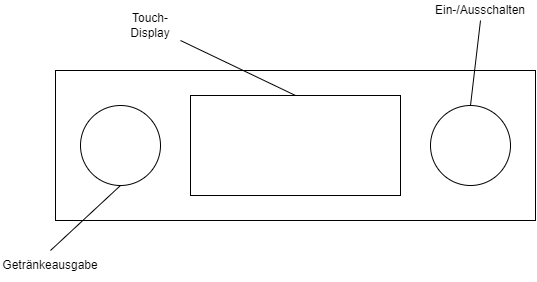
\includegraphics[width=0.8\textwidth]{img/Bilder_Stand_der_Technik/Bedienungsschnittstelle_Mischmaschine.png}}
    \caption{Schematischer Aufbau der Bedienungsschnittstelle}
    \label{fig:bedienungsschnittstelle_mischmaschine}
\end{figure}
\noindent
Abbildung \ref{fig:bedienungsschnittstelle_mischmaschine} stellt den schematischen Aufbau der Bedienungsschnittstelle der Getränkemischmaschine für ein besseres Verständnis dar.\\\\
Die technische Umsetzung basiert auf der Kommunikation zwischen dem Touch-Display und einem, in der Getränkemischmaschine verbauten, Arduino, der anhand der Daten von der Benutzereingabe, die Pumpen steuert. Beim Drücken des Startknopfes werden das Display und der Arduino mit Strom versorgt, sodass sowohl das Display als auch der Arduino starten und mit der Ausführung des benutzerdefinierten Quelltextes beginnen. Auf dem Bediendisplay finden sich fünf Schieberegler - ein Schieberegler je Behälter - mit denen der Benutzer die Zusammensetzung seines Mischgetränks aus den fünf Behältern konfigurieren kann. Beim Drücken eines in der \ac{UI} des Displays dargestellten Knopfes werden die Werte der Schieberegler an den Arduino übertragen. Dieser rechnet die Prozentwerte der Schieberegler in Durchsatzraten für die Pumpen um. Wird anschließend der Knopf für die Getränkeausgabe gedrückt gehalten steuert der Arduino die Pumpen mit ihrer jeweiligen Durchsatzrate an und der Anwender bekommt sein Mischgetränk ausgegeben.\\\\
Neben den bereits genannten Komponenten besitzt die Mischmaschine außerdem einen Wasserstandssensor je Behälter, um ein Trockenlaufen der Pumpen zu verhindern. Wie die einzelnen Komponenten zusammenspielen ist in dem Anhang \ref{Anhang_D} zu sehen, der den schematischen Aufbau/Schaltplan der Getränkemischmaschine zeigt \cite{mischmaschine}.
\section{Hardware}
\subsection{Arduino}
\subsubsection{Allgemeines}
Arduino ist eine Plattform/Organisation, die sich der Herstellung von Mikrocontrollern und der für den Umgang mit der Hardware erforderlichen Software widmet. Darunter fallen in erster Linie die Arduino-IDE und -Sprache zur Programmierung der Arduino-Mikrocontroller. Arduino verfolgt das Ziel, Hardwareprogrammierung oder \ac{IT} im Allgemeinen für alle Menschen unabhängig ihres Hintergrunds zu ermöglichen und näher zu bringen - allen voran auch denjenigen, die sich nicht professionell mit \ac{IT} auseinandersetzen \cite{arduino_education}. Deshalb liegt der Fokus von Arduino auf preisgünstigen Mikrocontrollern und einer einfachen Handhabung. Arduino stellt zu diesem Zweck auch viele Lernmaterialien bereit, die bspw. von Lehrkräften verwendet werden können als auch eine Community-Plattform für den Wissensaustausch zwischen den Benutzern von Arduino Hard- und Software. Pläne für die Arduino-Boards werden unter der \textit{Creative Commons} Lizenz veröffentlicht, sodass sie von anderen nachgebaut oder erweitert werden können. Auch der Quelltext der Arduino-Software ist quelloffen.
\subsubsection{Arduino-Programmierung}
Die Programmierung eines Arduino-Mikrocontrollers erfolgt über die Arduino-IDE \cite{arduino_ide}. Die Arduino-IDE kann auf allen gängigen Betriebssystemen (Windows, Mac und Linux) installiert und verwendet werden, was den Umgang mit Arduino sehr flexibel und gut für Einsteiger macht, da sie ihre gewohnte Umgebung verwenden können. Die Arduino-IDE ist dabei angelehnt an andere, gängige Entwicklungsumgebungen, sodass sich erfahrene Programmierer sofort zurecht finden, ist aber auf die Arduino-Programmierung optimiert. Beispielsweise werden an den Computer angeschlossene Boards automatisch erkannt, per Knopfdruck kann der aktuelle Quelltext auf den Mikrocontroller hochgeladen werden und die evtl. zusätzlich benötigten C++-Bibliotheken können verwaltet werden. Neben der Desktop-Version kann die Arduino-Entwicklungsumgebung auch online im Browser verwendet werden. Abbildung \ref{img:arduino_ide} zeigt einen Ausschnitt der Benutzeroberfläche in der Arduino-Entwicklungsumgebung.
\begin{figure}[H]
    \centering
    \fbox{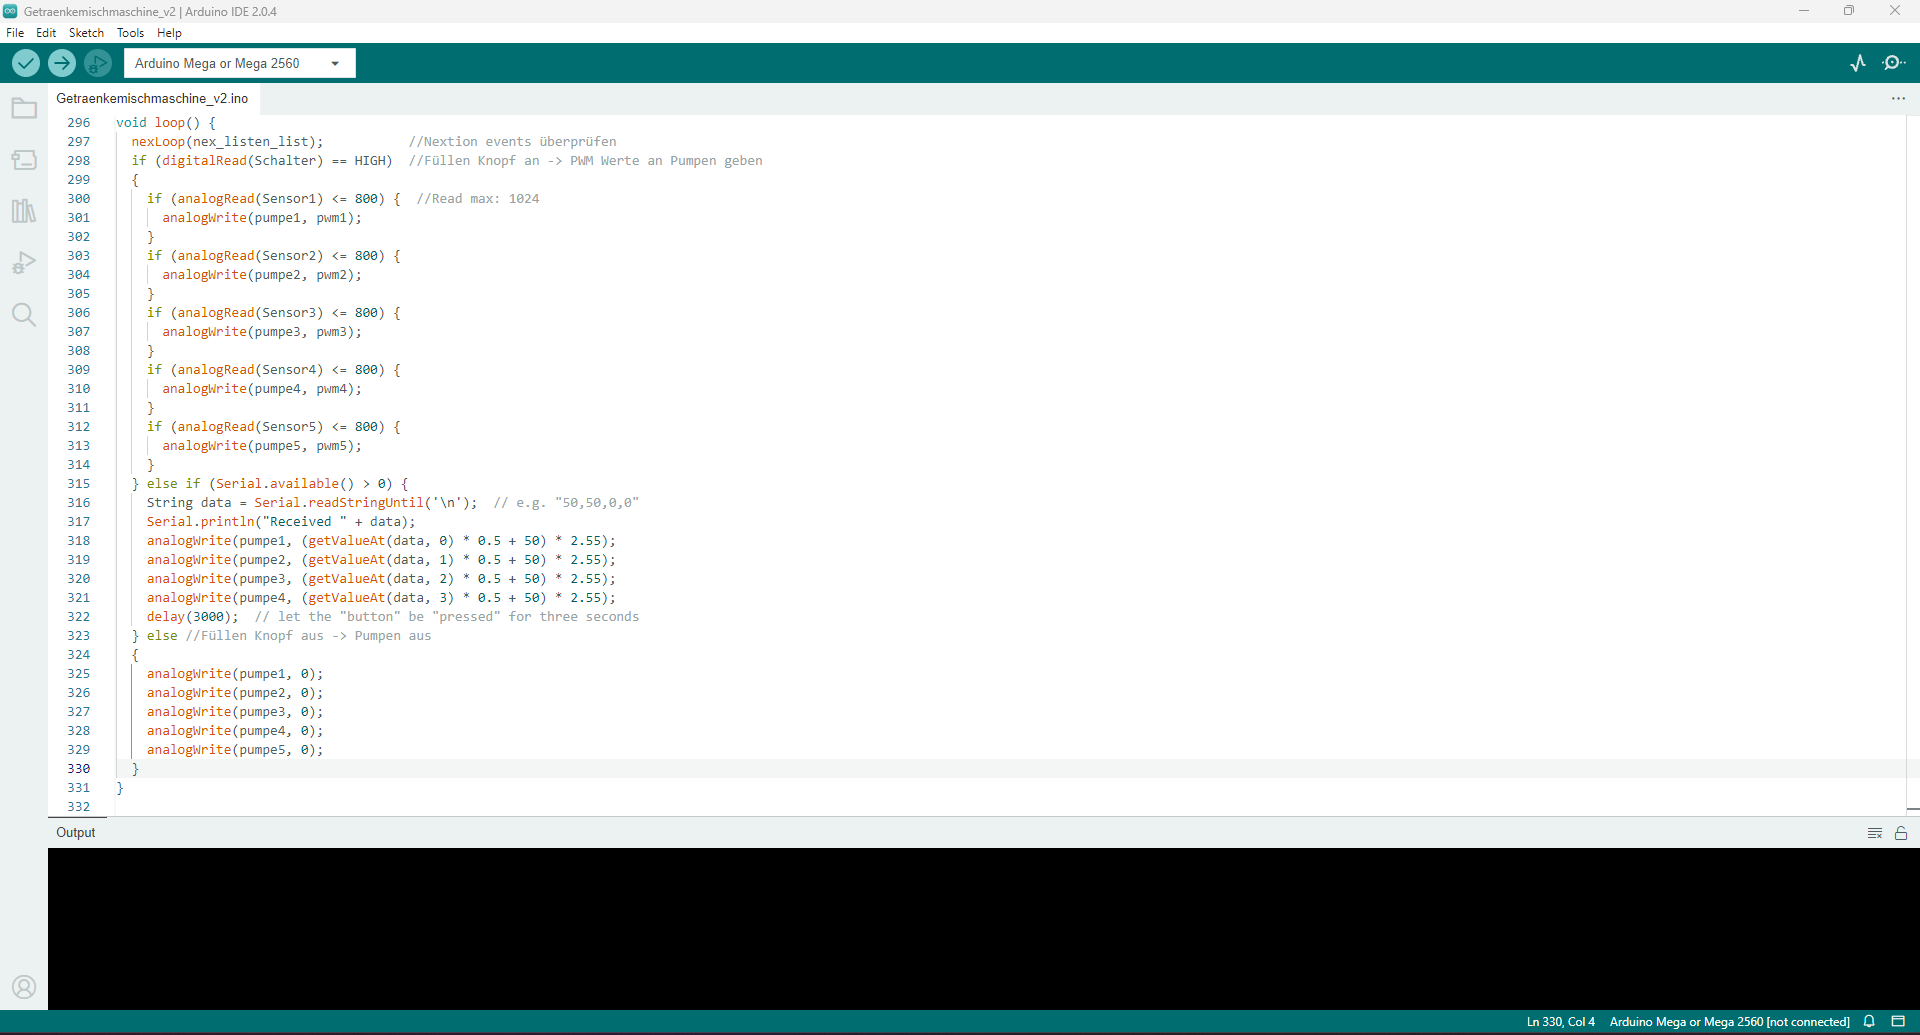
\includegraphics[width=\textwidth]{./img/Bilder_Stand_der_Technik/arduino_ide.png}}
    \caption{Arduino-IDE}
    \label{img:arduino_ide}
\end{figure}
\noindent
Ein Arduino-Mikrocontroller wird programmiert, indem das Programm in der Arduino-IDE und -Sprache geschrieben wird. Anschließend kann der Mikrocontroller über die USB-Schnittstelle an den Computer angeschlossen und der Quellcode durch Knopfdruck in der Entwicklungsumgebung an den Mikrocontroller gesendet werden, der sofort mit der Ausführung des Programms beginnt. Die meisten Mikrocontroller unterstützen kein Debugging um den Entwickler bei der Programmierung und Fehlersuche zu unterstützen. Manche Modelle verfügen jedoch über einen in Hardware implementierten Debugger zu diesem Zweck, der ebenfalls über die Entwicklungsumgebung verwendet werden kann.\\\\
Die Arduino-Programmiersprache ist angelehnt an \textit{Wiring} \cite{wiring} und kann durch eigene C++-Bibliotheken erweitert werden. Die Programmstruktur ist fest vorgegeben. Jedes Arduino-Programm besteht aus einer \textit{setup} und einer \textit{loop} Funktion. Die \textit{setup} Funktion wird exakt einmal zu Beginn des Programms aufgerufen, also wenn der Arduino mit Strom versorgt wird. Die \textit{loop} Funktion stellt die Hauptbefehlsschleife dar und enthält den Code, der den Großteil der Programmlogik enthält. Sie wird in einer Dauerschleife immer wieder neu aufgerufen. Listing \ref{arduino_example} stellt den Aufbau eines Arduino-Programms dar.\\
\lstinputlisting[language=c++, style=algoBericht, label={arduino_example}, basicstyle=\tiny\sffamily, captionpos=b, caption={Aufbau eines Arduino-Programms}]{./Listings/example.ino}
Die Arduino-Sprache stellt einige Sprachelemente bereit, die den Umgang mit der zugrundeligenden Hardware ermöglichen und erleichtern. Mit Sprachelementen sind sowohl innerhalb des Codes zugreifbare, globale Funktionen als auch Objekte gemeint. Abgesehen von \textit{setup} und \textit{loop} sind die wichtigsten Sprachelemente \cite{arduino_language}: 
\begin{itemize}
    \item \textit{HIGH} und \textit{LOW}: Diese beiden Konstanten werden verwendet, um den Wert eines digitalen Pins zu setzen. Wenn ein \textit{INPUT}-Pin mit \textit{digitalRead} gelesen wird, wird dieser die Konstante \textit{HIGH} zurückgeben, falls die Spannung, die an dem Pin anliegt, größer ist als 3V (bzw. größer als 2V bei einer Betriebsspannung von 3.3V) und \textit{LOW}, falls die Spannung kleiner ist als 1.5V (bzw. kleiner als 1V bei einer Betriebsspannung von 3.3V). Wenn ein \textit{OUTPUT}-Pin durch \textit{digitalWrite} auf \textit{HIGH} gesetzt wird, ist die anliegende Spannung am Pin gleich der Betriebsspannung des Arduino und 0V, falls der Wert \textit{LOW} geschrieben wird. 
    \item \textit{INPUT} und \textit{OUTPUT}: Diese beiden Konstanten werden verwendet um mit \textit{pinMode} das Verhalten eines Pins innerhalb des elektrischen Schaltkreises zu beeinflussen. \textit{INPUT}-Pins sind empfindlicher gegenüber Änderungen im elektrischen Schaltkreis, was sie geeignet zum Lesen von Sensorwerten macht. \textit{OUTPUT}-Pins können verwendet werden um andere Schaltkreise mit Strom zu versorgen.
    \item \textit{digitalRead(pin)} und \textit{digitalWrite(pin, value)}: Wird verwendet um einen der digitalen Ein-/Ausgabe-Pins des Arduinos zu Lesen oder zu Schreiben. Dabei können nur die Werte 0 oder 1 bzw. \textit{LOW} oder \textit{HIGH} gelesen und geschrieben werden. Das Argument \textit{pin} bezieht sich auf die Nummer des Pins, auf den zugegriffen werden soll.
    \item \textit{pinMode(pin, mode)}: Diese Funktion wird meist in der \textit{setup} Routine eines Arduino-Programms verwendet und registriert einen bestimmten Pin als \textit{INPUT} oder als \textit{OUTPUT} Pin, d.h. als Pin, der entweder lesend oder schreibend zugegriffen wird. Das bedeutet jedoch nicht, dass ein \textit{INPUT}-Pin nicht geschrieben werden oder ein \textit{OUTPUT}-Pin nicht gelesen werden darf. Ein als \textit{INPUT} deklarierter Pin hat lediglich sehr geringe Anforderungen an die Stromstärke, um seinen momentanen Wert zu ändern, sodass er sich besonders gut eignet um bspw. Sensorwerte abzulesen. Dadurch sind \textit{INPUT}-Pins auch empfindlicher gegenüber elektrischem Rauschen. \textit{OUTPUT}-Pins haben hingegen die Fähigkeit andere elektrische Geräte mit Strom zu versorgen, wie bspw. eine Leuchtdiode, da sie wesentliche Stromstärke nach Außen hin abgeben können.   
    \item \textit{analogRead(pin)} und \textit{analogWrite(pin, value)}: Diese beiden Funktionen können, im Gegensatz zu \textit{digitalRead} und \textit{digitalWrite}, verwendet werden um analoge Werte, d.h. Werte die in einem bestimmten Bereich liegen und sich von 0 und 1 unterscheiden können, zu lesen und zu schreiben. \textit{pin} bezieht sich hierbei auf die Nummer eines der analogen Pins des Arduino-Mikrocontrollers. Die verfügbare Auflösung ist von Modell zu Modell unterschiedlich. Die Auflösung bestimmt die Genauigkeit, mit der der Konverter die anliegenden Spannungen zwischen null und der Betriebsspannung des Arduinos (5V oder 3.3V) in Integer-Werte übersetzt. Der Konverter der meisten Arduino-Boards übersetzt die anliegende Spannung mit zehn Bit, d.h. in einen Integer-Wert von null bis 1024. Es gibt auch Konverter mit einer Auflösung von 12 Bit. Die Auflösung bestimmt also auch die Größe des Wertebereichs, in den übersetzt wird. Beim Schreiben eines analogen Wertes bestimmt \textit{value} den Taktzyklus des rechtwinkligen Wellensignals, das über den Pin gesendet wird und kann zwischen den Werten null und 255 liegen. Bei einem Zyklus von null degeneriert der Aufruf von \textit{analogWrite} zu einem Aufruf von \textit{digitalWrite(LOW)}, was bedeutet, dass kein Signal ausgegeben wird (die anliegende Spannung ist dauerhaft null). Bei einem Wert von 255 liegt hingegen dauerhaft Spannung an dem Pin an, was einem \textit{digitalWrite(HIGH)} entspricht. Abbildung \ref{img:pwm} zeigt die Auswirkungen auf das Signal je eingegebenem Wert \cite{pwm}. Man spricht in diesem Kontext von einer \glqq{}Pulsweitenmodulation\grqq{}, da ein wiederkehrendes Signal mit digitalen Mitteln (Signal an, Signal aus) modelliert wird. 
    \item \textit{delay(ms)}: Verzögert die Ausführung des Programms um \textit{ms} Millisekunden.
    \item \textit{Serial}: Neben den analogen und digitalen Pins besitzt jeder Arduino mindestens einen seriellen Port, um mit Computern und anderen Geräten zu kommunizieren. Neben dem obligatorischen USB-Hub, der vor allem dafür verwendet wird, um Programmcode auf den Mikrocontroller zu laden, haben die meisten Arduino-Boards weitere serielle TX/RX Pins. Dabei entspricht das \glqq{}T\grqq{} dem \glqq{}Transmitter\grqq{} und das \glqq{}R\grqq{} dem \glqq{}Receiver\grqq{}. Um diese Pins zur seriellen Kommunikation zu verwenden muss der TX-Pin am Arduino mit dem RX-Pin und der RX-Pin am Arduino mit dem TX-Pin des anzuschließenden Geräts verbunden werden. Um im Programmcode auf die seriell übertragenen Daten zuzugreifen wird das \textit{Serial}-Objekt verwendet, das wiederum weitere Methoden zur Verfgung stellt, um auf den Daten zu operieren. Um zwischen den verschiedenen seriellen Ports zu unterscheiden gibt es außerdem mehrere Objekte. \textit{Serial} bezieht sich auf den Standardport, d.h. entweder die Daten, die über den USB-Anschluss empfangen und gesendet werden oder auf die Pins 0(RX) und 1(TX). Das Objekt \textit{Serial1} kann verwendet werden um die Kommunikation über die Pins 19(RX) und 18(TX) zu steuern, das \textit{Serial2}-Objekt über die Pins 17(RX) und 16(TX) und so weiter. Natürlich unterscheiden sich die Pin-Nummern und verfügbaren Pins je nach Modell.
    \begin{itemize}
        \item \textit{Serial.available()}: Gibt die Anzahl von Bytes zurück, die sich bereits im seriellen Eingabepuffer befinden. Der serielle Eingabepuffer kann ein Maximum von 64 Bytes speichern.
        \item \textit{Serial.begin(speed)} oder \textit{Serial.begin(speed, config)}: Wird verwendet um die Übertragungsgeschwindigkeit zur seriellen Datenübertragung festzulegen. Es ist wichtig, dass die hier konfigurierte, sog. \glqq{}Baud-Rate\grqq{}, die selbe ist, wie auf dem Gerät, mit dem kommuniziert wird, da ansonsten Daten korrumpiert werden. \textit{speed} gibt die Geschwindigkeit der Datenübertragung in Bits pro Sekunde an. Mit dem optionalen \textit{config}-Argument können Daten-, Paritäts- und Stopp-Bits konfiguriert werden.
        \item \textit{Serial.println(val)} oder \textit{Serial.println(val, format)}: Wird verwendet um Daten an das Empfangsgerät über die serielle Schnittstelle zu senden. Schreibt die durch \textit{val} spezifizierten Daten als Strom von ASCII-Zeichen in den seriellen Ausgabepuffer. An \textit{val} werden automatisch ein Zeilenumbruch und ein Zeilenzeichen angehängt. Das optionale \textit{format}-Argument kann verwendet werden, um die Zahlenbasis (dezimal, hexadezimal, oktal oder binär) oder die Anzahl an Nachkommastellen (bei Fließkommazahlen) festzulegen.
        \item \textit{Serial.write(val)}, \textit{Serial.write(str)} oder \textit{Serial.write(buf, len)}: Im Unterschied zu \textit{Serial.print} oder \textit{Serial.println} wird \textit{Serial.write} verwendet, um Binärdaten über die serielle Schnittstelle an das Empfangsgerät zu senden. Es können sowohl einzelne Bytes (\textit{val}), Strings in Form eines Bytestroms (\textit{str}) als auch eine bestimmte Anzahl von Werten (\textit{len}) eines Byte-Arrays (\textit{buf}) übertragen werden.
        \item \textit{Serial.readStringUntil(terminator)}: Diese Funktion wird verwendet, um die Zeichen aus dem Eingabepuffer bis zu einem \textit{terminator}-Zeichen zu lesen und in einen String zu konvertieren. Es ist möglich einen Timeout zu konfigurieren, nach dem die Methode abbricht.
    \end{itemize}
\end{itemize}
\begin{figure}[H]
    \centering
    \fbox{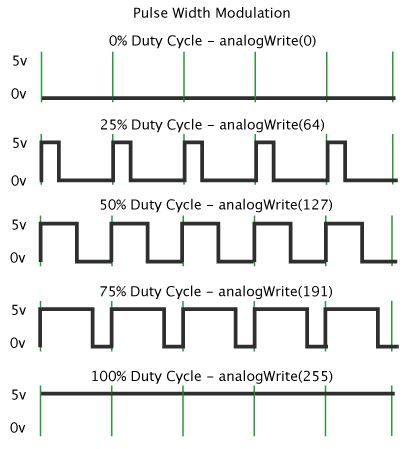
\includegraphics[width=0.8\textwidth]{./img/Bilder_Stand_der_Technik/pwm.png}}
    \caption{Pulsweitenmodulation}
    \label{img:pwm}
\end{figure}
\subsubsection{Elegoo Mega 2560 R3}
Bei dem \textit{Elegoo Mega 2560 R3} handelt es sich um einen Nachbau des Arduino Mega 2560 R3 \cite{arduino_mega}, der Firma \textit{Elegoo} \cite{elegoo}. Der \textit{Elegoo Mega 2560 R3} ist der, in der Mischmaschine eingebaute, Mikrocontroller und soll im Folgenden kurz vorgestellt werden.\\\\
Der \textit{Mega 2560} ist eine Mikrocontroller-Platine mit 54 digitalen Ein-/Ausgabe-Pins, 16 analogen Pins, von denen 15 zur Ausgabe einer Pulsweitenmodulation genutzt werden können und vier seriellen Ports, sowie einer USB-Schnittstelle. Der Mikrocontroller von \textit{Elegoo} ist kompatibel mit der Arduino-Software, d.h. er kann mit der Arduino-Entwicklungsumgebung programmiert und die C++-Bibliotheken für den Arduino können ebenfalls verwendet werden. Fünf der 16 analogen Pins werden für die Wasserstandssensoren der Mischmaschine verwendet und fünf weitere zum Ansteuern der Pumpen. Zur Kommunikation mit dem Touch-Display der Mischmaschine kommen zwei serielle Ports zum Einsatz (TX und RX). Die USB-Schnittstelle wird zum Programmieren des Mikrocontrollers verwendet. Ein digitaler Pin wird zum Lesen des Schalters zur Getränkeausgabe benutzt. Der \textit{Mega 2560} kann entweder über ein USB-Kabel oder über die ausgewiesenen Pins mit Strom versorgt werden. Die Mischmaschine verwendet die folgenden Pins zur Stromversorgung:
\begin{itemize}
    \item \textit{Vin}: Versorgt die Platine und den Mikrocontroller mit Spannung, die von dem Netzteil der Mischmaschine ausgeht. Das Spannungsnetz kann mit dem Hauptschalter vorne an der Mischmaschine geschlossen oder unterbrochen werden.
    \item \textit{5V}: Dieser Pin gibt eine Spannung von 5V nach Außen ab und versorgt damit das Touch-Display der Mischmaschine.
    \item \textit{GND} eins und zwei: Pins für die Erdung.
\end{itemize} 
Der Mikrocontroller, der sich auf der Platine befindet, ist der \textit{ATmega2560}, der mit einer Taktrate von 16 \ac{MHz} arbeitet, d.h. es können 16 Millionen Berechnungen pro Sekunde ausgeführt werden. Der \textit{ATmega2560} beinhaltet einen vorprogrammierten Bootloader, sodass neuer Programmcode ohne externen Programmierer auf den Mikrocontroller geladen werden kann. Die Betriebsspannung beträgt 5V.
\subsection{Nextion}
\subsubsection{Allgemeines}
\textit{Nextion} beschäftigt sich mit dem Vertrieb und der Herstellung von \textit{Human Machine Interface} (HMI) Lösungen \cite{zhou_home_nodate}. Darunter sind Touch-Displays mit eingebautem Prozessor und Arbeitsspeicher zu verstehen und der \textit{Nextion Editor}, welcher die Programmierung von Benutzeroberflächen erleichtern soll, indem Grafiken, Text, Knöpfe, Slider und andere Komponenten via drag-and-drop angeordnet werden können. Die HMI-Displays von \textit{Nextion} kommunizieren über eine serielle Schnittstelle mit den peripherie Geräten, an die sie angeschlossen werden sollen. Es werden nur ein 5V-Anschluss, Erdung und die TX-/RX-Pins benötigt. Das Display wird über eine Menge von ASCII-basierten Instruktionen gesteuert.\\\\
Das Angebot von \textit{Nextion} ist in vier Modellreihen aufgeteilt: \textit{Intelligent Series}, \textit{Enhanced Series}, \textit{Discovery Series} und \textit{Basic Series}. Die \textit{Intelligent Series} beinhaltet die leistungssträksten Displays mit mehr Rechenleistung und Speicher im Vergleich zur \textit{Enhanced} oder \textit{Basic Series}. Außerdem können Displays aus dieser Serie andere Komponenten in der Benutzeroberfläche darstellen. Die \textit{Basic Series} beinhaltet die preisgünstigsten Modelle von \textit{Nextion}.
\subsubsection{NX4832T035}
In der Mischmaschine ist ein \textit{Nextion}-Display vom Typ NX4832T035, aus der \textit{Basic Series}, eingebaut \cite{nx4832t035}. Das Display besitzt eine Größe von 3.5 Zoll und eine Bildschirmauflösung von 480 mal 320 Pixeln.\\\\
Wie bereits erwähnt wurde wird zur Programmierung der Benutzeroberfläche der \textit{Nextion Editor} verwendet. Der \textit{Nextion Editor} erlaubt es sog. HMI-Projekte zu erstellen, welche die Benutzeroberfläche und alle damit verbundenen Ressourcen (benutzerdefinierter Code, Bilder, Videos, ...) enthalten. Wie auch bei Arduino wird das \textit{Nextion}-Display über eine serielle Schnittstelle programmiert, über die das HMI-Projekt vom Entwicklungscomputer auf das Display geladen werden kann. Die Oberfläche wird bei \textit{Nextion} aus ein oder mehreren Seiten zusammengesetzt, die wiederum Komponenten verschiedenster Art, wie bspw. Knöpfe, Slider oder Textfelder, enthalten können. Jede Komponente hat eine Reihe von Attributen, wie bspw. x-y-Koordinaten, Farben oder eine eindeutige Kennung, die konfigurierbar sind. Die Komponenten und Seiten können bestimmte Events abfeuern. Zwei häufig verwendete Events sind \glqq{}Touch Press\grqq{} und \glqq{}Touch Release\grqq{}, die abgefeuert werden, wenn der Benutzer einen bestimmten bereich mit seinem Finger berührt oder loslässt. Abbildung \ref{img:nextion_editor_overview} zeigt die Oberfläche des Nextion-Editors. Die dargestellte Seite ist die Startseite, auf der der Benutzer zur Wartungsseite wechseln kann, um die Mischmaschine zu administrieren oder mit der Auswahl der Getränke fortfahren kann.
\begin{figure}[H]
    \centering
    \fbox{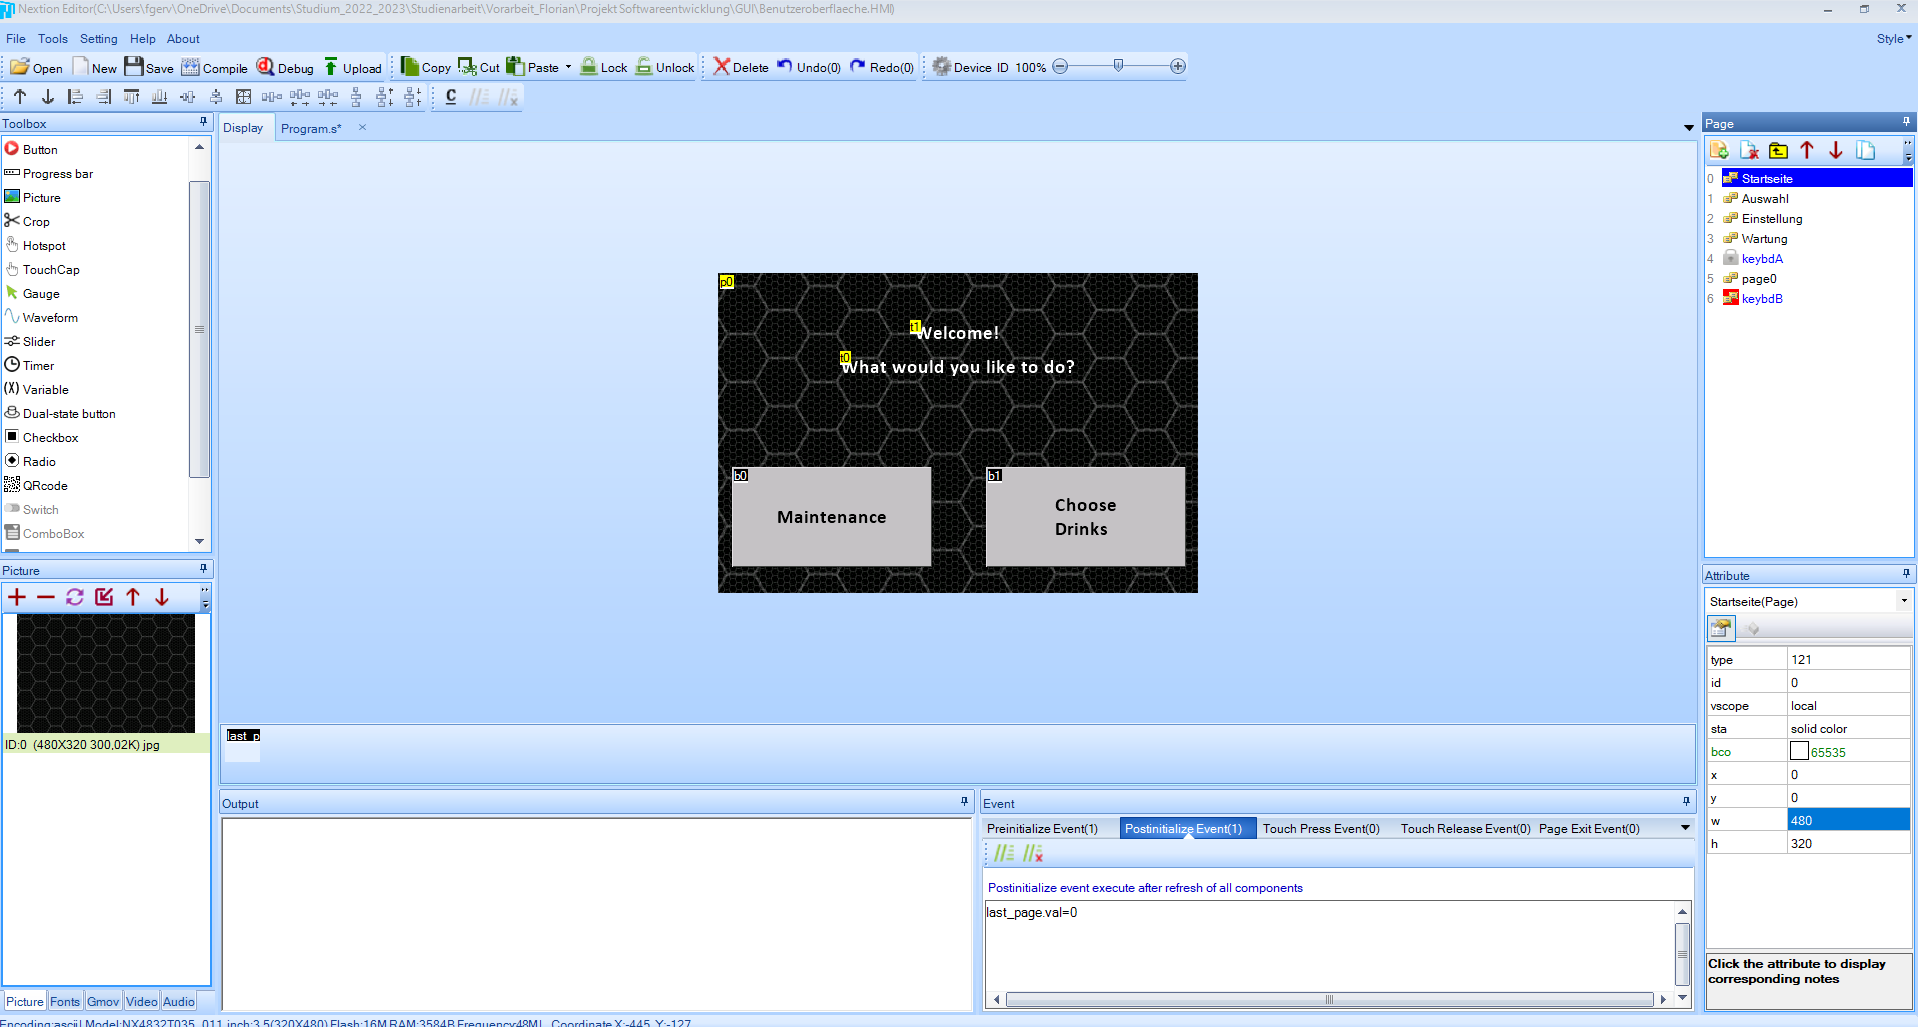
\includegraphics[width=0.95\textwidth]{./img/Bilder_Stand_der_Technik/nextion_editor_overview.png}}
    \caption{Überblick über den Nextion-Editor}
    \label{img:nextion_editor_overview}
\end{figure}
\noindent
Die Events, die von der aktuell ausgewählten Komponente abgefeuert werden, werden im Editor dargestellt. Unterhalb davon befindet sich ein Textbereich, in den direkt Quellcode geschrieben werden kann, der bei Auftreten des Events ausgeführt wird. Der Quellcode besteht aus einer Abfolge von Instruktionen aus dem \textit{Nextion}-Befehlssatz \cite{nextion_instructions}.\\\\
Zur Kommunikation zwischen Display und Peripheriegerät (hier der Elegoo Mega) existieren Bibliotheken für Arduino und Raspberry Pi. Für dieses Projekt wird die Arduino-Bibliothek verwendet \cite{nextion_library}. Dabei handelt es sich um eine C++-Bibliothek, die zu einem Arduino-Programm als Abhängigkeit hinzugefügt und mit \textit{\#include<Nextion.h>} eingebunden werden kann. Für die \textit{Nextion}-Komponenten gibt es entsprechende Klassen, wie bspw. \textit{NexButton}, \textit{NexCheckbox} oder \textit{NexPage}. Die Bibliothek kann über die Konfigurationsdatei \glqq{}NexConfig.h\grqq{}, bei der es sich um eine simple C-Header-Datei handelt, konfiguriert werden, indem die dort definierten Konstanten abgeändert werden. Hier lässt sich bspw. der Wert der Konstanten \textit{\#define nexSerial Serial2} ändern, um zu bestimmen, über welche seriellen Ports die Kommunikation mit dem Display stattfinden soll. Um die Benutzung der Arduino-\textit{Nextion}-Bibliothek zu veranschaulichen ist in Listing \ref{nextion_example} ein einfaches Beispielprogramm zu sehen.\\
\lstinputlisting[language=c++, style=algoBericht, label={nextion_example}, basicstyle=\tiny\sffamily, captionpos=b, caption={Beispielprogramm mit Nextion}, escapeinside={//*}{*)}]{./Listings/nextion.ino}
Innerhalb des Programms ist es notwendig, alle Komponenten, auf deren Events reagiert werden soll, einer Liste hinzuzufügen. Dies passiert in den Zeilen \ref{code:begin_nex_touch_list} bis \ref{code:end_nex_touch_list}. Die Liste besteht aus Objekten vom Typ \textit{NexTouch}, welche die Vaterklasse aller \textit{Nextion}-Komponenten ist, die auf Touch-Events reagieren können. Diese Liste wird der \textit{nexLoop}-Methode übergeben, die innerhalb der Arduino \textit{loop}-Methode aufgerufen werden muss (s. Zeile \ref{code:nexLoop}). Daraufhin werden die deklarierten Komponenten immer wieder auf neue Events überprüft. In diesem Beispiel ist die einzige Komponente ein Button. Dieser nimmt im Konstruktor drei Argumente entgegen: die eindeutige Kennung \glqq{}0\grqq{} der Seite, auf der sich die Komponente befindet, die eindeutige Kennung \glqq{}1\grqq{} der Komponente selbst sowie ihr Name \glqq{}b0\grqq{}. Um auf das Event eines konkreten Objektes zu reagieren wird mit einem Aufruf der \textit{attachPop}-Methode eine Callback-Funktion für eine bestimmte Komponente übergeben, die bei einem \glqq{}Pop Touch\grqq{} aufgerufen wird. Daneben gibt es auch noch die \textit{attachPush}-Methode, um auf ein \glqq{}Push Touch\grqq{} Event zu reagieren. In diesem Beispiel wird die \textit{b0PopCallback}-Methode, die in Zeile \ref{code:b0PopCallback} deklariert wird, als Callback für den Button in Zeile \ref{code:attachPop} verwendet.
\begin{figure}[H]
    \centering
    \fbox{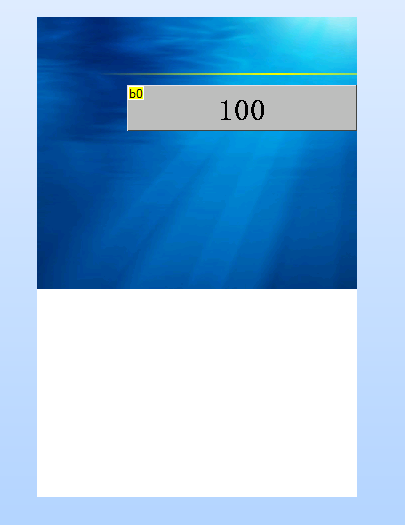
\includegraphics[height=0.5\linewidth]{./img/Bilder_Stand_der_Technik/nextion_example.png}}
    \caption{Benutzeroberfläche des Beispielprogramms im \textit{Nextion}-Editor}
    \label{img:nextion_example}
\end{figure}
\noindent
Abbildung \ref{img:nextion_example} zeigt die Oberfläche der Beispielanwendung. Der Callback sorgt dafür, dass der Text innerhalb der Button-Komponente nach jedem Klick um eins inkrementiert wird. Dafür wird in Zeile \ref{code:cast} das Argument der Callback-Funktion vom Typ \textit{void*} zu einem \textit{NexButton}-Objekt konvertiert. Die Variable \textit{ptr} hält nämlich eine Referenz auf das Objekt des Callbacks, sodass anschließend der Text des Buttons mit \textit{getText} in den zuvor definierten Puffer geladen werden kann. Der Inhalt des Puffers wird in eine Zahl konvertiert (Zeile \ref{code:to_int_conversion}), um eins inkrementiert und schließlich als neuer Text der Button-Komponente gesetzt (Zeile \ref{code:setText}).\\\\
Das Display sendet die Events der Komponenten über die serielle Schnittstelle an das Peripheriegerät (hier der Elegoo Mega) in Form eines ASCII-codierten Zeichenstroms. Ebenso kann das Display vom Client aus gesteuert werden, indem Befehle aus der umfangreichen Menge von Instruktionen über die serielle Schnittstelle an das Display gesendet werden, um auf Events zu reagieren.
\subsection{Raspberry Pi} \label{section:raspberry}
\subsubsection{Allgemeines}
Die Raspberry Pi Foundation beschäftigt sich mit dem Vertrieb und der Herstellung der namensgebenden Raspberry Pi Minicomputer und Mikrocontroller, sowie der benötigten Software und Zubehör. Dabei verfolgt Raspberry Pi das selbe Ziel wie Arduino, nämlich einer möglichst großen Gruppe von Menschen Informatik näher zu bringen und sie zu befähigen mit ihrem erworbenen Wissen, eigene Projekte umzusetzen. Deshalb gelten die Raspberry Pi Computer als sehr preisgünstig und es existieren große Mengen von Lernmaterialien für Lehrkräfte oder für das Selbststudium. \cite{raspberry_home}\\\\
Raspberry Pi entwickelt für seine Computer das eigene Betriebssystem \glqq{}Raspberry Pi OS\grqq{}. Dieses gibt es in verschiedenen Versionen. Die \glqq{}Lite\grqq{}-Version beinhaltet bspw. keine Desktop-Umgebung. Das Betriebssystem ist sowohl in 32- als auch 64-Bit verfügbar. Auch andere Betriebssysteme lassen sich auf der Raspberry-Hardware installieren, wie bspw. das weit verbreitete Linux-Derivat \glqq{}Ubuntu\grqq{}. Neben dem für die Raspberry Pi Hardware optimierten Raspberry Pi OS gibt es auch eine Version für allgemeine Computer-Hardware oder Apple-Geräte.
\subsubsection{Der Raspberry Pi 4 Modell B}
Der Raspberry Pi Computer, der in dieser Arbeit zum Einsatz kommt, ist der Raspberry Pi 4 Modell B. Bei dem Raspberry Pi 4 handelt es sich um die gegenwärtig aktuellste Version des Minicomputers. Er ist in vier verschiedenen Ausführungen erhältlich, die sich jeweils in dem verfügbaren Arbeitsspeicher unterscheiden: 1 \ac{GB}, 2 \ac{GB}, 4 \ac{GB} und 8 \ac{GB}. Hier kommt das Modell mit 4 \ac{GB} zum Einsatz.\\\\
Desweiteren besitzt der Raspberry Pi 4 zwei USB 3.0 sowie zwei USB 2.0 Ports, Gigabit Ethernet, Bluetooth 5.0 und einen WLAN-Chip zur Kommunikation mit anderen Geräten - auch über das Internet. Wichtig ist auch der Steckplatz für die Micro SD Karte, die zum Laden des Betriebssystems und Persistieren von Daten unverzichtbar ist. Der eingebaute Prozessor kann Datenworte von einer Länge von 64 Bit verarbeiten und Berechnungen mit einer Geschwindigkeit von 1.5 \ac{GHz} durchführen. Der Raspberry Pi 4 unterstützt das betreiben von zwei 4K-Monitoren gleichzeitig über die zwei Mikro-HDMI-Ports.\\\\
\begin{figure}[H]
    \centering
    \fbox{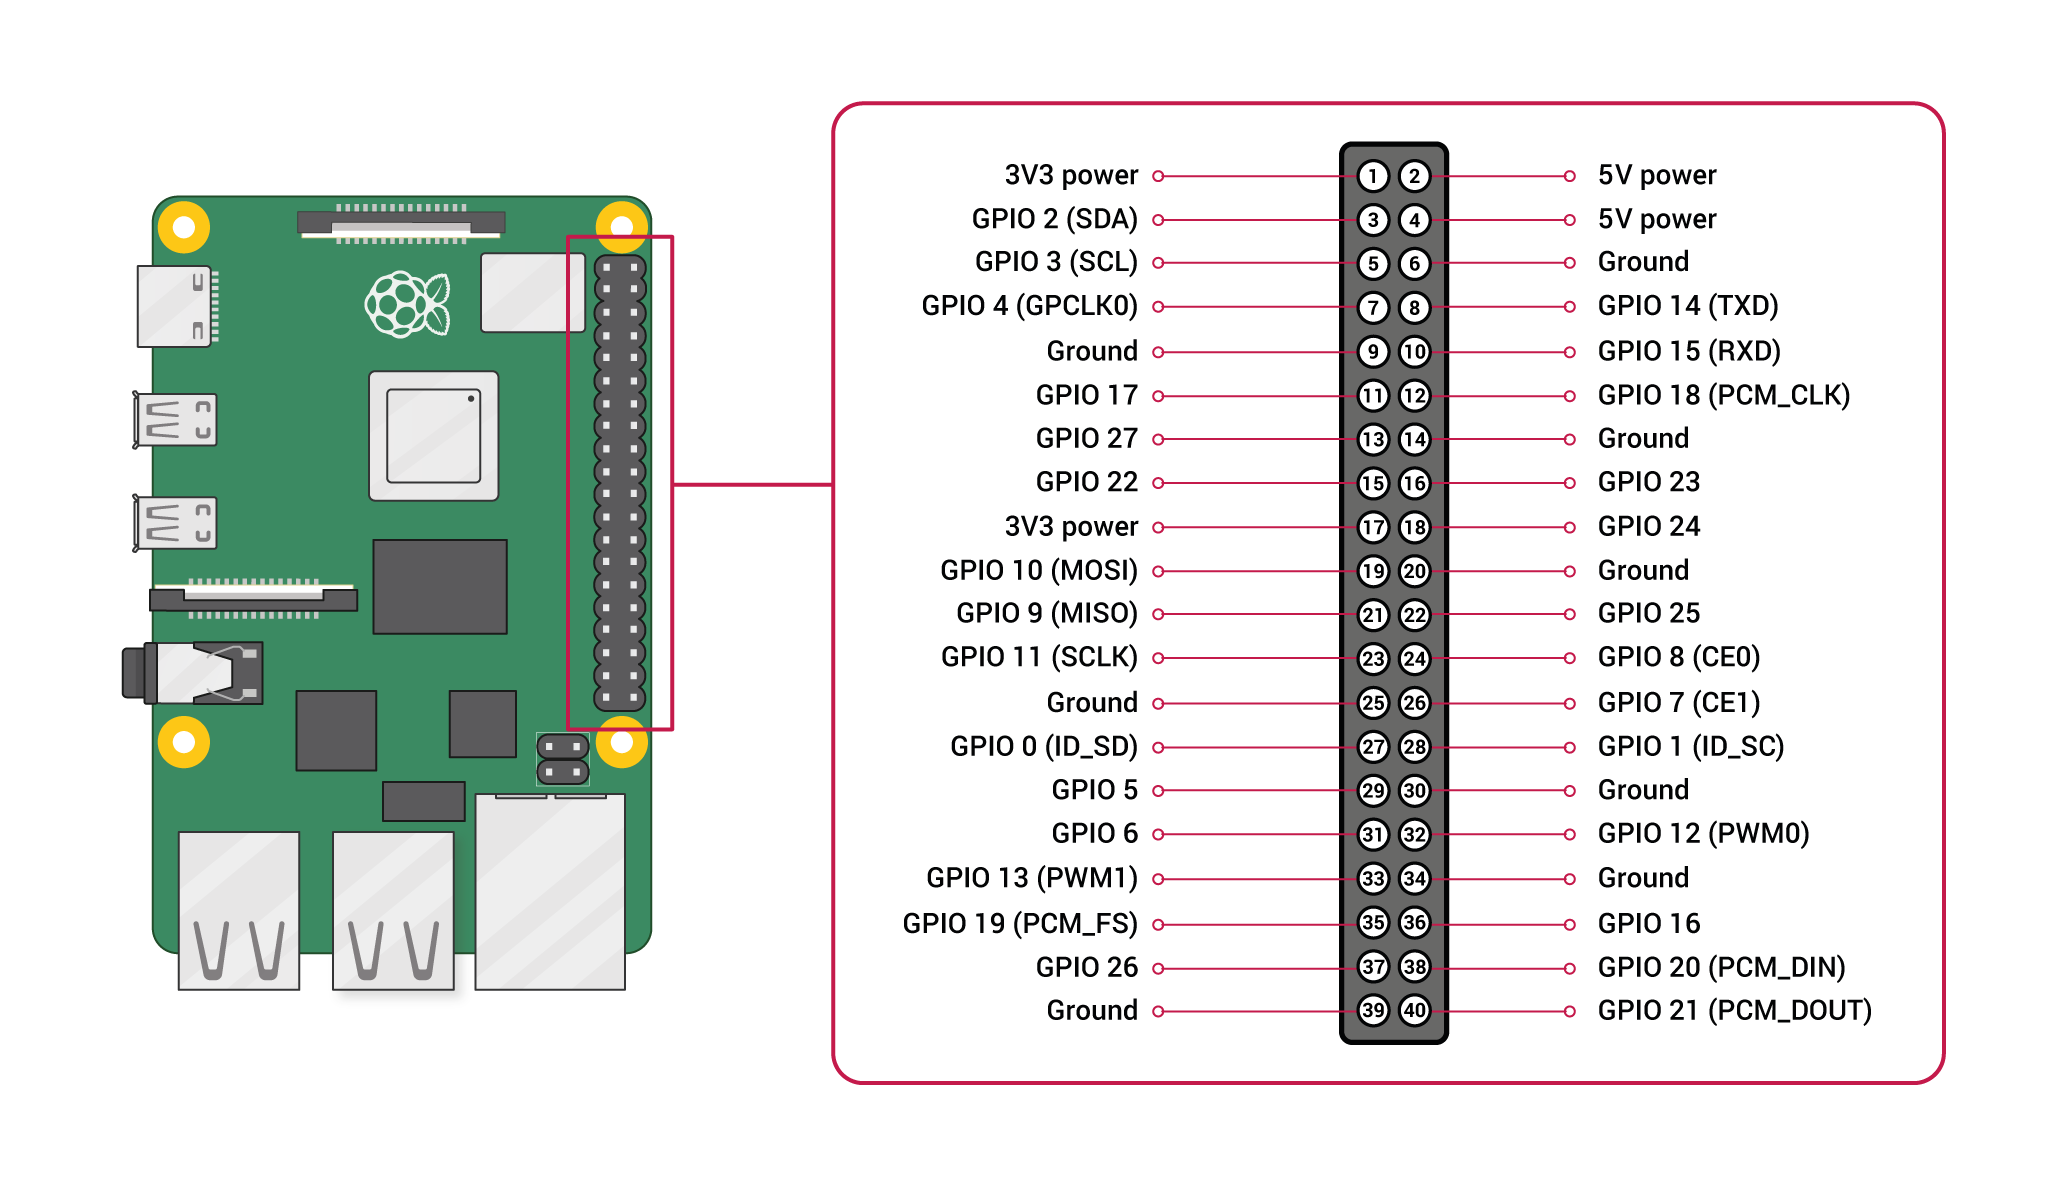
\includegraphics[width=0.8\textwidth]{./img/Bilder_Stand_der_Technik/pinout_raspberry.png}}
    \caption{GPIO-Pinout für den Raspberry Pi 4}
    \label{img:pinout_raspberry}
\end{figure}
\noindent
Neben den oben genannten Schnittstellen besitzt der Raspberry Pi 4 zusätzlich 40 \ac{GPIO} Pins, die in Abbildung \ref{img:pinout_raspberry} zu sehen sind \cite{raspberry_doc}. Unter den Pins finden sich zwei 5V Pins, sieben Ground-Pins (0V), zwei serielle Pins und vier Pins, die Hardware-Pulsweitenmodulation unterstützen. Die restlichen Pins sind normale \ac{GPIO}-Pins, die auf 3.3V operieren, d.h. als Ausgabe ausgeweisene Pins können auf low (0V) oder high (3.3V) gesetzt werden und ein als Eingabe ausgewiesener Pin kann als low (0V) oder high (3.3V) gelesen werden. Um die Pins über Software zu kontrollieren bietet sich die \textit{GPIO Zero} Python-Bibliothek an \cite{gpiozero}. 
\section{Sprachverarbeitung}
Im Zuge des technologischen Fortschritts nutzen die Menschen heutzutage zunehmend Sprachassistenten für verschiedene Aufgaben. 
Einer der Hauptvorteile der Sprachsteuerung ist die Bequemlichkeit und Geschwindigkeit, mit der Aufgaben erledigt werden können, ohne dass man tippen oder mit der Maus klicken muss. 
Sprachassistenten nutzen die Verarbeitung natürlicher Sprache, um Befehle zu erkennen und zu verstehen, die der Nutzer laut ausspricht.\\\\
Die Verarbeitung natürlicher Sprache - \ac{NLP} - ist eine wichtige Technologie, die es Computern ermöglicht, die von Menschen verwendete natürliche Sprache zu verstehen. 
Diese Technologie ermöglicht es Computern, menschliche Sprache zu erkennen und zu interpretieren und Text und Sprache in natürlicher Sprache zu erzeugen. 
Im Bereich der Sprachsteuerung spielt \ac{NLP} eine Schlüsselrolle bei der Erkennung von Sprache und dem Verstehen von Befehlen, die der Benutzer laut ausspricht. 
Es wird verwendet, um die Sprache des Benutzers in Text umzuwandeln, den ein Computer verstehen und verarbeiten kann.
Um dies zu erreichen, verwendet \ac{NLP} eine Vielzahl von Techniken und Technologien, darunter maschinelles Lernen, Tonanalyse, syntaktische Analyse und mehr. \cite{jurafsky_speech_2009}\\\\
Im Rahmen dieses Projekts erfordert die Implementierung der Sprachsteuerung einer Getränkemischmaschine die Verarbeitung natürlicher Sprache, damit die Maschine Befehle verstehen kann, die der Benutzer laut ausspricht. 
Dieses Projekt ähnelt einem Chatbot, bei dem der Benutzer eine Frage stellen oder einen Befehl geben kann und der Chatbot führt die entsprechende Aktion aus. 
Die Verarbeitung natürlicher Sprache ist für die Entwicklung eines solchen Sprachsteuerungssystems unerlässlich und ermöglicht es der Maschine, Befehle in natürlicher Sprache zu verstehen und auszuführen.\\\\
Eine der wichtigsten Komponenten der Verarbeitung natürlicher Sprache ist die Spracherkennung und das Syntaxanalyseverfahren. 
Bei der Spracherkennung kommen Deep-Learning-Techniken zum Einsatz, die es einem Computer ermöglichen, Sprachlaute zu erkennen und in Text zu übersetzen. 
Anschließend wird das Syntaxanalyseverfahren verwendet, um die Satzstruktur zu bestimmen und Schlüsselwörter und -sätze hervorzuheben, die zur Bestimmung des Benutzerbefehls verwendet werden können.
Auch die Tonwertanalyse ist ein wichtiger Bestandteil der Verarbeitung natürlicher Sprache. 
Mit Hilfe der Tonalitätsanalyse lässt sich die emotionale Färbung des Textes bestimmen, was für die Ermittlung der Absicht des Nutzers nützlich sein kann. 
Da die Tonwertanalyse im Rahmen dieser Arbeit nicht relevant ist, wird sie nicht weiter erörtert. \cite{jurafsky_speech_2009}\\\\
Darüber hinaus werden grammatik- und regelbasierte Technologien zur Verarbeitung natürlicher Sprache eingesetzt. 
Diese Technologien werden eingesetzt, um die korrekte Struktur des Benutzerbefehls zu bestimmen und Schlüsselwörter hervorzuheben, die zur Durchführung von Aktionen verwendet werden können. 
Außerdem werden Techniken des maschinellen Lernens eingesetzt, damit der Computer aus früheren Befehlen und Aktionen \glqq{}lernen\grqq{} kann, was die Genauigkeit der Erkennung von Benutzerbefehlen verbessert.\\\\
Daher ist der Einsatz von Technologien zur Verarbeitung natürlicher Sprache für das Projekt der Sprachmischmaschine unerlässlich. 
Die Verarbeitung natürlicher Sprache wird es der Maschine ermöglichen, die Befehle zu verstehen und zu verarbeiten, die der Benutzer laut ausspricht und die entsprechenden Aktionen durchzuführen.
\subsection{Verarbeitung natürlicher Sprache}
Die Verarbeitung natürlicher Sprache ist ein Forschungsbereich der Informatik und der \ac{KI}, der sich mit der Verarbeitung natürlicher Sprache befasst. 
Bei der Verarbeitung geht es in der Regel darum, natürliche Sprache in Daten zu übersetzen, die ein Computer nutzen kann, um Informationen über die Welt um ihn herum zu erhalten.\\\\
Die \ac{NLP}-Pipeline, die zur Erstellung eines Dialogsystems erforderlich ist, erfordert vier Arten der Verarbeitung sowie eine Datenbank zur Speicherung vergangener Äußerungen und Antworten. 
Jeder dieser Schritte kann einen oder mehrere Verarbeitungsalgorithmen enthalten, die parallel oder sequentiell arbeiten \cite{lane_natural_2019}:
\begin{itemize}
    \item Syntaktische Zergliederung - Extraktion von Merkmalen (strukturierte numerische Daten) aus natürlichem Text.
    \item Analyse - Erstellen und Kombinieren von Items, um Indikatoren für den Ton, die grammatikalische Korrektheit und die Semantik des Textes zu erhalten.
    \item Generierung - Generierung möglicher Antworten mit Hilfe von Mustern, Suchwerkzeugen oder Sprachmodellen.
    \item Ausführung - bereitet Aussagen vor, die auf der Geschichte und dem Zweck des Gesprächs basieren und wählt eine Folgeantwort.
\end{itemize}
\begin{figure}[H]
    \centering
    \fbox{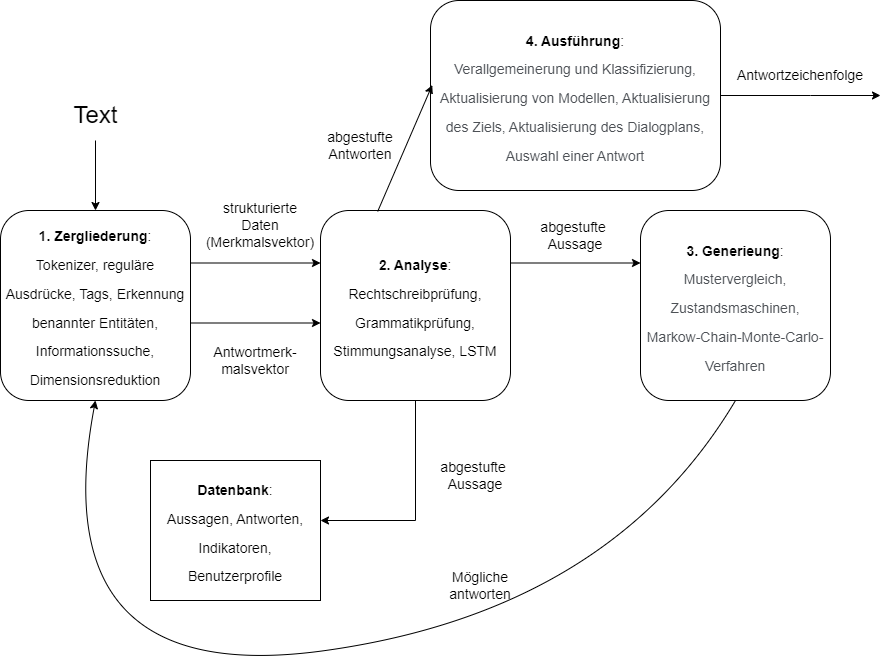
\includegraphics[width=0.8\textwidth]{Bilder_Stand_der_Technik/Chat-Bot-Pipeline.png}}
    \caption{Rekurrente Chat-Bot-Pipeline}
    \label{figure:Chat-Bot-Pipeline}
\end{figure}
\noindent
Die meisten Chatbots enthalten Elemente aus allen fünf Teilsystemen (die vier Verarbeitungsstufen sowie die Datenbank). 
Viele Anwendungen erfordern jedoch nur einfache Algorithmen, um viele dieser Schritte auszuführen. 
Ein Chatbot oder virtueller Assistent für Verbraucher wie Alexa oder Allo ist in der Regel so konzipiert, dass er äußerst sachkundig und leistungsfähig ist. 
Die Logik, die zur Beantwortung von Anfragen verwendet wird, ist jedoch oft oberflächlich und besteht aus einer Reihe von Codephrasen, die mit einer einzigen if-then-Entscheidungsverzweigung zur gleichen Antwort führen. 
Alexa (und die zugrundeliegende Lex-Engine) verhält sich wie ein einschichtiger, flacher Baum von Operatoren (if, elif, elif...). 
Andererseits stützt sich die Google Translate-Pipeline (oder jedes ähnliche maschinelle Übersetzungssystem) auf eine mehrstufige Hierarchie von Merkmalsextraktoren, Entscheidungsbäumen und Wissensgraphen, die Fragmente von Wissen über die Welt miteinander verbinden. \cite{janarthanam_hands-chatbots_2017}\\\\
Alle \ac{NLP}-Merkmale müssen gut funktionieren, damit das Dialogsystem richtig funktioniert \cite{lane_natural_2019}:
\begin{itemize}
    \item Merkmalsextraktion (normalerweise zur Erstellung eines Vektorraummodells).
    \item Informationssuche zur Beantwortung von Sachfragen.
    \item Semantische Suche, um Informationen aus zuvor aufgezeichneten natürlichsprachlichen Texten oder Dialogen zu assimilieren.
    \item Generierung von natürlicher Sprache, um neue sinnvolle Aussagen zu verfassen.
\end{itemize}
\subsection{Tokenisierung von Wörtern}
Eine der wichtigsten Aufgaben der Verarbeitung natürlicher Sprache ist die Tokenisierung, d. h. die Zerlegung von Text in einzelne Wörter oder Phrasen, die so genannten Token. 
Dieser Prozess ist ein wichtiger Bestandteil der Verarbeitung natürlicher Sprache, da er es Programmen und Algorithmen ermöglicht, Texte anhand ihrer Bestandteile zu verstehen und zu analysieren. 
Die Tokenisierung ist für die Verarbeitung natürlicher Sprache von entscheidender Bedeutung, da sie es Programmen ermöglicht, Schlüsselwörter, Phrasen und semantische Einheiten in einem Text hervorzuheben. 
Die Tokenisierung kann auch dazu verwendet werden, nicht benötigte Textelemente wie Satzzeichen, Leerzeichen und andere Zeichen, die keine Bedeutung haben, zu entfernen. 
Dadurch können Programme und Algorithmen effizienter und genauer arbeiten und die Wahrscheinlichkeit von Fehlern und falscher Textverarbeitung verringern. \cite{jurafsky_speech_2009}\\\\
Im \ac{NLP} ist die Tokenisierung eine besondere Art der Segmentierung von Dokumenten. 
Bei der Segmentierung wird der Text in kleinere Abschnitte (Segmente) mit engerem Informationsgehalt unterteilt. 
Die Segmentierung kann die Aufteilung eines Dokuments in Absätze, in Sätze, in Phrasen und in Token (Wörter) sowie Satzzeichen umfassen. 
Ein Tokenizer kann mit einem Scanner im Kompilierungsprozess verglichen werden. 
Token sind in diesem Fall die Endpunkte von kontextfreien Grammatiken - \ac{CFG} - zur Analyse von Programmiersprachen-Terminalen. \cite{bird_natural_2009}\\\\
Die Tokenisierung ist der erste Schritt in der \ac{NLP}-Pipeline und kann daher den Rest der Pipeline stark beeinflussen. 
Der Tokenizer zerlegt unstrukturierte Daten, d. h. natürlichsprachliche Texte, in Informationseinheiten, die als einzelne Elemente gezählt werden können. 
Die so gezählte Anzahl von Token-Vorkommen in einem Dokument kann direkt als Vektor verwendet werden, der dieses Dokument repräsentiert. 
Ein solcher Ansatz ermöglicht es, aus einer unstrukturierten Zeichenfolge (einem Textdokument) unmittelbar eine für das maschinelle Lernen geeignete numerische Datenstruktur zu gewinnen. 
Diese Werte können den Computer direkt dazu veranlassen, nützliche Aktionen durchzuführen und Reaktionen zu erzeugen. \cite{lane_natural_2019}\\\\
Die einfachste Art, einen Satz zu tokenisieren, ist die Verwendung von Leerzeichen als Worttrenner in Zeichenketten. 
Dies ist jedoch nicht optimal, denn wenn ein Satz z. B. ein Satzzeichen enthält, wird es von einem der Tokenisierer erfasst. 
Optimierte Tokenizer sind in mehreren Python-Bibliotheken implementiert, die jeweils ihre eigenen Vor- und Nachteile haben: spaCy, Stanford CoreNLP und \ac{NLTK}. 
\ac{NLTK} und StanfordCoreNLP sind die am längsten bestehenden und am häufigsten verwendeten Bibliotheken zum Vergleich von \ac{NLP}-Algorithmen in wissenschaftlichen Artikeln. 
Obwohl die StanfordCoreNLP-Bibliothek eine Python-\ac{API} hat, basiert sie auf dem Java 8 CoreNLP-Anwendungsteil, der separat installiert und konfiguriert werden muss. 
Daher wurde in dieser Arbeit der \ac{NLTK}-Tokenizer verwendet.\\\\
Ein wichtiges Konzept im Tokenisierungsprozess sind N-Gramme. 
Ein N-Gramm ist eine Sequenz mit bis zu n Elementen, die aus einer Sequenz dieser Elemente, in der Regel einer Zeichenkette, extrahiert wurden. 
Im Allgemeinen können die Elemente eines N-Gramms Buchstaben, Silben, Wörter oder sogar Symbole sein. 
N-Gramme sind notwendig, weil bei der Konvertierung einer Menge von Wörtern in einen Vektor eine Folge von Token einen Großteil der Bedeutung verliert, die in der Reihenfolge dieser Wörter verkapselt ist. 
Wenn das Token-Konzept auf Mehrwort-Token, N-Gramme, ausgedehnt wird, kann die \ac{NLP}-Pipeline einen erheblichen Teil der Bedeutung, die in der Wortfolge dieser Äußerungen enthalten ist, beibehalten. 
So bleibt beispielsweise das Wort \glqq{}kein\grqq{}, das die Bedeutung umkehrt, neben den benachbarten Wörtern stehen, wo es hingehört. 
Ohne N-Gramm-Tokenisierung würde ein solches Wort an verschiedenen Positionen herumhängen und seine Bedeutung würde mit dem gesamten Satz oder Dokument assoziiert werden, anstatt mit benachbarten Wörtern. 
Das Bigramm \glqq{}war nicht\grqq{} behält viel mehr Bedeutung der einzelnen Wörter \glqq{}war\grqq{} und \glqq{}nicht\grqq{} als die entsprechenden Singlegramme im Multigrammvektor. 
Durch die Verknüpfung eines Wortes mit seinen Nachbarn in einem Förderband kann ein Teil seines Kontexts erhalten bleiben. 
N-Gramme sind also ein Instrument zur Speicherung von Kontextinformationen, während die Daten die Pipeline durchlaufen. \cite{lane_natural_2019}\\\\
Die Größe des Vokabulars spielt eine wichtige Rolle für die Leistung der \ac{NLP}-Pipeline. 
Die Größe des Wörterbuchs bestimmt die Größe der Trainingsstichprobe, die benötigt wird, um eine Überanpassung an ein bestimmtes Wort oder eine bestimmte Phrase zu vermeiden und die Größe der Trainingsmenge bestimmt die Kosten der Verarbeitung. 
Eine Technik zur Verringerung der Größe des Wörterbuchs besteht darin, Token, die ähnliche Dinge bedeuten, in einer einzigen normalisierten Form zusammenzufassen. 
Eine solche Technik reduziert die Anzahl der gespeicherten Token und verbessert die Verbindungen zwischen den Bedeutungen von Phrasen mit unterschiedlicher \glqq{}Schreibweise\grqq{} der Tokens und verringert die Wahrscheinlichkeit des Überlernens. 
Eine der Normalisierungsmöglichkeiten ist die Groß- und Kleinschreibung - die Kombination mehrerer Schreibweisen eines Wortes, die sich nur in der Groß- und Kleinschreibung unterscheiden. 
In diesem Fall wird die Groß-/Kleinschreibung ignoriert und zwei identische Wörter, von denen eines groß und das andere klein geschrieben wird, werden als dasselbe Token behandelt.\\\\
Ein weiterer wichtiger Schritt bei der Tokenisierung von Texten ist die Entfernung von Stoppwörtern, um den Umfang des Wörterbuchs zu verringern. 
Stoppwörter sind in jeder Sprache gebräuchliche Wörter, die sehr häufig vorkommen, aber sehr viel weniger aussagekräftige Informationen über die Bedeutung eines Satzes enthalten (z. B. a, an, the, this, of, on im Englischen oder der, die, das, diese im Deutschen). 
Stoppwörter können jedoch nützliche Informationen enthalten, so dass man sie nicht immer verwerfen sollte. 
Das \ac{NLTK}-Paket für Python enthält derzeit die umfassendste Liste kanonischer Stoppwörter in verschiedenen Sprachen. \cite{mccarthy_applied_2011}\\\\
Eine weitere gängige Methode der Normalisierung ist die Beseitigung kleiner semantischer Unterschiede im Zusammenhang mit Pluralendungen und Possessivendungen von Wörtern oder sogar unterschiedlichen Verbformen. 
Diese Methode der Normalisierung, bei der ein gemeinsamer Wortstamm für verschiedene Wortformen gefunden wird, wird als Stemming bezeichnet. 
Der gemeinsame Wortstamm von \glqq{}Gehäuse\grqq{} und \glqq{}Haus\grqq{} ist zum Beispiel \glqq{}Haus\grqq{}.
 Beim Stemming werden Suffixe von Wörtern entfernt, um Wörter mit ähnlicher Bedeutung unter einem gemeinsamen Stamm zu gruppieren. 
 Der Wortstamm muss nicht unbedingt ein gültiges Wort sein, sondern kann auch nur ein Token oder eine Bezeichnung sein, das mehrere mögliche Schreibweisen repräsentiert. 
 Einer der Hauptvorteile des Stemming besteht darin, die Anzahl der Wörter zu verringern, deren Bedeutung das Sprachmodell im Auge behalten muss. 
 Durch diese Methode wird die Größe des Wörterbuchs reduziert, wodurch der Verlust nützlicher Informationen und Bedeutungen so weit wie möglich begrenzt wird. 
 Das Stemming spielt eine wichtige Rolle bei der Suche nach Schlüsselwörtern oder Informationen. 
Zwei der bekanntesten Algorithmen sind Porter's Stemmer und Snowball. \cite{manning_foundations_1999}\\\\
Mit Informationen über die Beziehungen zwischen den Bedeutungen verschiedener Wörter ist es möglich, mehrere Wörter miteinander zu verknüpfen, auch wenn ihre Schreibweise sehr unterschiedlich ist. 
Eine solche erweiterte Normalisierung eines Wortes auf seine semantische Wurzel - ein Lemma - wird Lemmatisierung genannt. 
Die Lemmatisierung ist potenziell eine viel genauere Art der Normalisierung als das Stemming oder die Groß- und Kleinschreibung, da sie die Bedeutung des Wortes berücksichtigt. 
Der Lemmatisierer verwendet eine Wissensbasis von Synonymen und Wortendungen, um nur eng verwandte Wörter zu einem Token zu kombinieren. 
In Python kann die Lemmatisierung mit dem \ac{NLTK}-Paket implementiert werden, das den \textit{WordNetLemmatizer} enthält. \cite{nltk_wordnet}\\\\
Wie bereits gezeigt wurde, ist die Tokenisierung der Prozess der Zerlegung von Text in einzelne Wörter oder Token. 
Für viele Anwendungen der Verarbeitung natürlicher Sprache ist jedoch nicht nur wichtig, welche Wörter im Text enthalten sind, sondern man muss auch in der Lage sein, diese Wörter als Zahlen darzustellen. 
Dadurch wird es möglich, maschinelles Lernen und andere Algorithmen, die mit Zahlen arbeiten, zur Textverarbeitung einzusetzen. 
Bei der Verarbeitung natürlicher Sprache wird dazu die Wortvektorisierung verwendet.
\subsection{Vektorisierung von Wörtern}
Die Vektorisierung hilft dabei, eine numerische Darstellung zu finden, die die Bedeutung oder den Informationsgehalt der dargestellten Wörter widerspiegelt. 
Es gibt drei Möglichkeiten, Wörter und ihre Bedeutungen darzustellen \cite{lane_natural_2019}:
\begin{itemize}
    \item Multisets von Wörtern - Vektoren von Zahlen oder Häufigkeiten von Wörtern. 
    \item Multisets von N-Grammen - Vektoren von Mengen von Wortpaaren (Bigramme), Worttripeln (Trigramme), usw.
    \item \ac{TF}-\ac{IDF}-Vektoren sind Indikatoren für Wörter, die deren Bedeutung am Besten darstellen.
\end{itemize}
Jede dieser Methoden kann entweder allein oder als Teil einer \ac{NLP}-Pipeline angewendet werden. 
Alle beschriebenen Modelle sind statistisch in dem Sinne, dass sie auf Worthäufigkeiten beruhen.
\subsubsection{Multisets von Wörtern}
\ac{BOW}-Vektoren sind Vektoren, die Textdokumente als Wort-Multisets (Bags) darstellen, wobei ein Multiset eine Sammlung von Elementen ist, in der jedes Element mehr als einmal wiederholt werden kann. 
Ein Wort-Bag ist eine Darstellung von Text, die das Vorkommen von Wörtern in einem Dokument beschreibt. 
Sie beinhaltet zwei Dinge:
\begin{enumerate}
    \item Ein Wörterbuch mit bekannten Wörtern.
    \item Ein Maß für das Vorhandensein von bekannten Wörtern.
\end{enumerate}
Dies wird als \glqq{}Word-Bag\grqq{} bezeichnet, weil alle Informationen über die Reihenfolge oder Struktur der Wörter im Dokument verworfen werden. 
Das Modell interessiert sich nur dafür, ob bekannte Wörter im Dokument vorkommen, nicht aber, wo im Dokument. 
Bei diesem Ansatz wird das Histogramm der Wörter im Text betrachtet, d. h. wir betrachten jedes Wort als ein Merkmal \cite{goldberg_neural_2017}.\\\\
Ein Ansatz zur Vektorisierung einer Vielzahl von Wörtern besteht darin, für jedes Wort einen Einheitsvektor zu erstellen und diese Vektoren dann zu einem einzigen Vektor zu kombinieren. 
Ein unitärer Vektor für ein Wort ist ein Vektor, dessen Länge der Dimension des Raumes entspricht und alle seine Komponenten sind Null, mit Ausnahme einer Komponente, die der Position des Wortes im Wörterbuch entspricht. Unitäre Vektoren sind extrem spärlich. 
Enthält das Wörterbuch beispielsweise 1000 Wörter, dann hat jeder unitäre Vektor eine Dimension von 1000 und die Komponente, die der Position des Wortes im Wörterbuch entspricht, ist gleich eins.
Zum Beispiel sieht der unitäre Vektor für den Satz \glqq Mojito ist ein leckerer Cocktail\grqq{} (nach dem Tokenisierungsprozess) so aus:
\begin{figure}[H]
    \centering
    \fbox{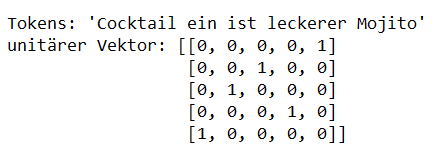
\includegraphics[width=0.6\textwidth]{Bilder_Stand_der_Technik/unitaerer_vektor.png}}
    \caption{\label{figure:Unitaere_Vektoe}Unitärer Vektor}
\end{figure}
\noindent
Eine der Eigenschaften der vektoriellen Darstellung von Wörtern und der tabellarischen Darstellung von Dokumenten ist, dass keine ursprünglichen Informationen verloren gehen. 
Das Originaldokument kann aus dieser einheitlichen Vektortabelle rekonstruiert werden \cite{bird_natural_2009}.
Daher werden solche unitären Vektoren in neuronalen Netzen, bei der \ac{seq2seq}-Modellierung und bei der Erstellung von Sprachmodellen verwendet. 
Unitäre Vektoren eignen sich hervorragend für alle \ac{NLP}-Modelle oder -Pipelines, bei denen die Bedeutung des Ausgangstextes vollständig erhalten bleiben muss.
Die Erstellung von unitären Vektoren für jedes Wort kann mit verschiedenen Bibliotheken in Python erfolgen. 
Zum Beispiel kann die NumPy-Bibliothek verwendet werden, um unitäre Vektoren zu erstellen. \cite{numpy}\\\\
Diese Vektordarstellung hat jedoch ihre Nachteile. 
Bei Dokumenten, die eine große Anzahl von Wörtern enthalten, wäre die Größe des unitären Vektorwörterbuchs enorm und würde enorme Ressourcen zur Verarbeitung erfordern. 
Außerdem macht es keinen Sinn, so viele Nullen zu speichern. 
Um mit dem Wörterbuch arbeiten zu können, ohne viel Zeit für die Verarbeitung zu verschwenden, ist es notwendig, das Wörterbuch zu verkleinern. 
Dazu ist es notwendig, auf die Möglichkeit der Rekonstuierung des Originaldokuments zu verzichten, d.h. sich die Wortfolge aller Dokumente zu merken. 
Es ist notwendig, den größten Teil der Informationen zu erfassen, nicht das gesamte Dokument. Dafür sind Multiset-Vektoren hilfreich.\\\\
Um einen Vektor für ein Multiset von Wörtern zu erstellen, müssen für jedes Wort der Mehrmenge ein Einheitsvektor erstellt und diese Vektoren dann zu einem einzigen Vektor kombiniert werden. 
Vektoren können nach verschiedenen Regeln kombiniert werden, z. B. durch Addition, Multiplikation, Verkettung oder andere Operationen. 
Wenn alle diese unitären Vektoren zusammengezählt werden, wird ein Vektor der Worthäufigkeit erhalten. 
Er spiegelt die Häufigkeit des Vorkommens von Wörtern wider, nicht die Reihenfolge, in der sie auftreten. 
Dieser Vektor kann verwendet werden, um ein ganzes Dokument oder einen Satz als einen einzigen Vektor von nicht sehr großer Länge darzustellen. 
Seine Länge entspricht der Länge des Wörterbuchs (der Anzahl der verfolgten eindeutigen Token). 
Außerdem kann bei einer einfachen Schlüsselwortsuche ein binärer Multiset-Vektor durch eine logische OR-Operation aus unitären Vektoren gewonnen werden. \cite{bird_natural_2009}\\\\
Die Anzahl der Vorkommen eines Wortes in einem bestimmten Dokument wird als Termfrequenz (\ac{TF}) bezeichnet \cite{lane_natural_2019}. 
Je häufiger ein Wort in einem Dokument vorkommt, desto wahrscheinlicher ist es, dass das Dokument von diesem Thema handelt. 
Anstelle von reinen Wortzählungen können auch normalisierte Termhäufigkeiten zur Beschreibung von Dokumenten aus einem Korpus verwendet werden. 
Unter normalisierten Dokumenthäufigkeiten versteht man die Anzahl der Wörter im Verhältnis zur Länge des Dokuments. 
Die Normalisierung ist sehr nützlich, um die Bedeutung eines Dokuments zu ermitteln, da reine Häufigkeiten nicht immer die tatsächliche Situation widerspiegeln. 
Wenn beispielsweise das Wort \glqq Cocktail\grqq{} 15 Mal in Dokument \textnumero 1 und 400 Mal in Dokument \textnumero 2 vorkommt, kann man daraus schließen, dass es in Dokument Nummer zwei eher um Cocktails geht.
Vielleicht handelt es sich aber bei Dokument \textnumero 1 um ein Rezept für die Zubereitung von Mai Tais mit 100 Wörtern, während Dokument \textnumero 2 ein Roman mit 500.000 Wörtern ist, in dem die Figuren gelegentlich Cocktails trinken. 
Die Häufigkeit des Wortes \glqq Cocktail\grqq{} in Dokument \textnumero 1 beträgt also 0,15 und 0,0008 in Dokument \textnumero 2, was die tatsächliche Bedeutung des Begriffs \glqq Cocktail\grqq{} in diesen Dokumenten viel besser widerspiegelt:
\begin{figure}[H]
    \centering
    \fbox{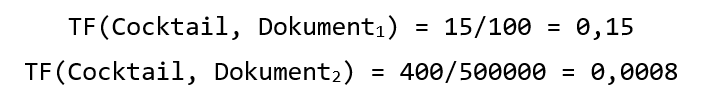
\includegraphics[width=0.8\textwidth]{Bilder_Stand_der_Technik/norm_vektoren.png}}
    \caption{\label{figure:Norm_Vektoren}Normalisierte TF-Vektoren}
\end{figure}
\noindent
Ebenso ist es möglich, diesen Wert für jedes Wort zu berechnen und die relative Bedeutung dieses Begriffs für jedes Dokument zu ermitteln, woraus sich die Bedeutung jedes Dokuments ableiten lässt. 
Um die Anzahl der Vorkommen von Wörtern zu ermitteln, kann das Objekt \textit{collections.Counter} in Python verwendet und anschließend eine Normalisierung durchgeführt werden:
\begin{figure}[H]
    \centering
    \fbox{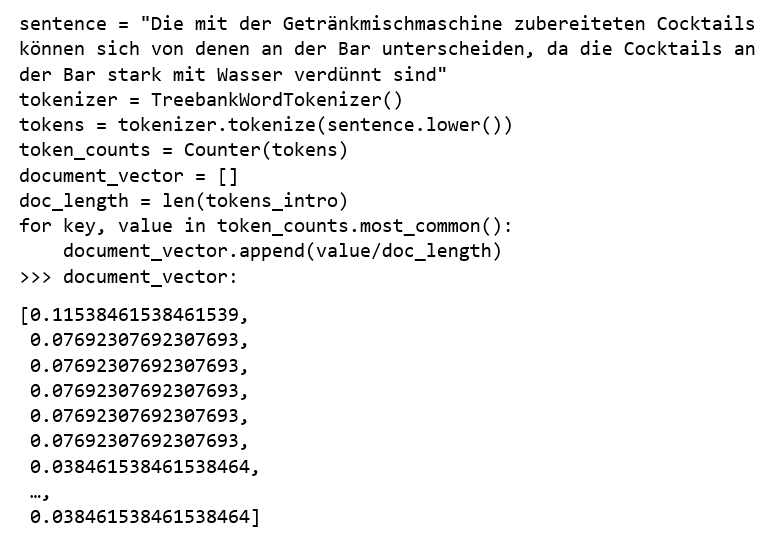
\includegraphics[width=0.8\textwidth]{Bilder_Stand_der_Technik/norm_vek_py.png}}
    \caption{\label{figure:Norm_Vektoren_Python}Normalisierte TF-Vektoren mit Python}
\end{figure}
\noindent
Wenn mehr als ein Dokument bearbeitet wird, wird für jedes Dokument ein eigener Häufigkeitsvektor erstellt, der jedoch absolut alle Begriffe aus allen Dokumenten (alle Wörter aus dem Wörterbuch) enthält, auch wenn einige der Wörter nicht in allen Dokumenten vorkommen. 
In diesem Fall werden die Vektoren an diesen Stellen Nullwerte enthalten.\\\\
Das ultimative Ziel der Textvektorisierung besteht darin, natürliche Sprache in ein Format zu übersetzen, das der Computer verstehen kann. 
Eine Möglichkeit, dies zu erreichen, ist die Verwendung von Vektorräumen. 
Vektorräume sind mathematische Objekte, in denen jedes Element durch einen Vektor dargestellt wird und verschiedene Operationen mit Vektoren ermöglichen es uns, nützliche Merkmale zu extrahieren. 
So wird ein Vektor mit zwei Werten in einem zweidimensionalen Vektorraum verortet, ein Vektor mit drei Werten in einem dreidimensionalen Vektorraum und so weiter. 
Beispielsweise ist der Vektorraum von Dokumenten, die nur aus den Wörtern \glqq Cocktail\grqq{} und \glqq Maschine\grqq{} bestehen, zweidimensional und die Vektoren der enthaltenen Dokumente können wie folgt dargestellt werden:
\begin{figure}[H]
    \centering
    \fbox{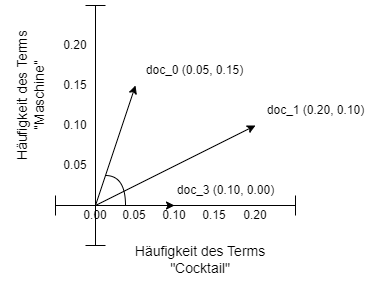
\includegraphics[width=0.6\textwidth]{Bilder_Stand_der_Technik/vraum.png}}
    \caption{\label{figure:Vraum}Zweidimensionale Vektoren von Termhäufigkeiten}
\end{figure}
\noindent
Für einen Vektorraum von Dokumenten in einer natürlichen Sprache ist die Dimensionalität des Vektorraums gleich der Anzahl der verschiedenen Wörter im gesamten Korpus. 
Jedes Dokument in einem K-dimensionalen Vektorraum kann durch einen K-dimensionalen Vektor beschrieben werden. 
Wenn es Vektorrepräsentationen für alle Dokumente im gleichen Raum gibt, dann ist es möglich, sie zu vergleichen. 
Der euklidische Abstand zwischen Vektoren kann gemessen werden, indem sie subtrahiert werden und die Länge des Abstands zwischen ihnen berechnet wird, den sogenannten Abstand im Sinne der L2-Norm (L2-Metrik). 
Dies ist der Abstand auf einer geraden Linie von dem Ort, der durch die Spitze (Scheitelpunkt) des einen Vektors gegeben ist, zu dem Ort, der der Spitze des anderen Vektors entspricht. \cite{weisstein_l2-norm_nodate}
\begin{equation}
    d(p, q) = ||q-p||_2 = \sqrt{(q_1 - p_1)^2 + ... + (q_n - p_n)^2} = \sqrt{\sum_{i=1}^{n} (q_i - p_i)^2}
    \eqlabel{eu-norm}{Euklidische Norm}
\end{equation}
Der Ochiai-Koeffizient (Kosinuskoeffizient) ist ein Maß für die Ähnlichkeit zwischen zwei Multisets. 
Der Ochiai-Koeffizient kann verwendet werden, um den Grad der Ähnlichkeit zwischen zwei Dokumenten auf der Grundlage ihrer Wort-Multisets zu bestimmen. 
Er ist einfach der Kosinus des Winkels zwischen zwei Vektoren (Theta). \cite{han_data_2011}
\begin{figure}[H]
    \centering
    \fbox{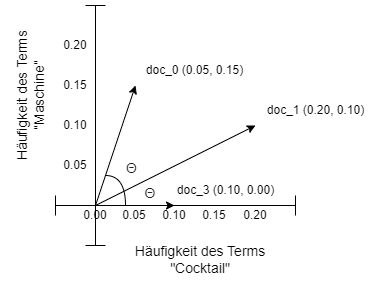
\includegraphics[width=0.6\textwidth]{Bilder_Stand_der_Technik/vraum_theta.png}}
    \caption{\label{figure:Vraum_Theta}Zweidimensionale Theta}
\end{figure}
\noindent
Er kann mithilfe des euklidischen Skalarprodukts nach folgender Formel berechnet werden:
\begin{equation}
    A \cdot B = ||A||\: ||B||\: cos\, \theta
    \eqlabel{eu-skal-prod}{Euklidisches Skalarprodukt}
\end{equation}
\begin{equation}
    cosine\: similarity = S_c(A, B) := cos( \theta) = \frac{A \cdot B}{||A||\: ||B||} =  \frac{\sum_{i=1}^{n} (A_i\: B_i)}{ \sqrt{\sum_{i=1}^{n} A_i^2}\: \sqrt{\sum_{i=1}^{n} B_i^2}}
    \eqlabel{och-coef}{Ochiai-Koeffizient}
\end{equation}
Das Skalarprodukt zweier Vektoren kann also berechnet werden, indem die Elemente der Vektoren paarweise multipliziert und dann die Ergebnisse addiert werden. 
Anschließend wird das Ergebnis durch die Norm jedes Vektors dividiert. 
Die Norm eines Vektors ist gleich dem euklidischen Abstand zwischen seinem Kopf und seinem Ende - der Quadratwurzel aus der Summe der Quadrate seiner Elemente. 
Dieses normierte Skalarprodukt liegt wie der Kosinuswert zwischen -1 und 1. 
Es ist auch der Kosinus des Winkels zwischen den beiden Vektoren. 
Dieser Wert ist gleich dem Anteil des längeren Vektors, der von der senkrecht dazu stehenden Projektion des kürzeren Vektors abgedeckt wird. 
Daraus ist ersichtlich, wie weit unsere beiden Vektoren in dieselbe Richtung zeigen.\\\\
Ein offensichtlicher Vorteil ist, dass der vom Ochiai-Koeffizienten angenommene Wertebereich (von -1 bis +1) für die meisten Aufgaben des maschinellen Lernens geeignet ist. 
Ein Kosinuskoeffizient von 1 spiegelt identische normalisierte Vektoren wider, die über alle Dimensionen hinweg in eine ähnliche Richtung zeigen. 
Die Längen dieser Vektoren können unterschiedlich sein, aber sie zeigen in dieselbe Richtung. 
Je näher der Kosinuskoeffizient bei 1 liegt, desto kleiner ist der Winkel zwischen den Vektoren.
Im \ac{NLP} enthalten Dokumente, deren Kosinuskoeffizient der Vektoren nahe bei 1 liegt, ähnliche Wörter im gleichen Verhältnis. 
Daher ist es wahrscheinlicher, dass es sich bei Dokumenten, deren Vektoren nahe beieinander liegen, um dieselbe Sache handelt. 
Wenn der Kosinuskoeffizient 0 ist, haben die Vektoren keine gemeinsamen Komponenten. 
Sie stehen in allen Dimensionen in einem 90°-Winkel zueinander. 
Bei \ac{TF}-\ac{NLP}-Vektoren tritt diese Situation nur ein, wenn die beiden Dokumente keine gemeinsamen Wörter haben. 
Da sie völlig unterschiedliche Wörter verwenden, sprechen sie von völlig unterschiedlichen Dingen. 
Das bedeutet nicht unbedingt, dass die Bedeutung oder das Thema unterschiedlich ist, sondern nur, dass sie unterschiedliche Wörter verwenden. 
Bei einem Wert des Kosinuskoeffizient von -1 sind die Vektoren völlig entgegengesetzt. 
Sie zeigen in entgegengesetzte Richtungen. 
Bei einfachen Vektoren der Termhäufigkeiten ist dies jedoch nicht möglich, da Vektoren der Termhäufigkeiten nicht negativ sein können. 
Sie befinden sich also immer im gleichen Quadranten des Vektorraums. \cite{han_data_2011}\\\\
Neben den Multisets von Wörtern gibt es weitere Vektorisierungsmethoden, die ebenfalls in der Verarbeitung natürlicher Sprache verwendet werden - Multisets von N-Grammen und \ac{TF-IDF}-Vektoren.
Bei Multisets von N-Grammen handelt es sich um Mengen von mehreren aufeinanderfolgenden Wörtern in einem Text. 
N-Gramme können helfen, den Kontext und die Beziehung zwischen Wörtern in einem Text zu erfassen. 
In diesem Fall wird nicht die Häufigkeit der einzelnen Begriffe im Dokument berücksichtigt, sondern die Häufigkeit des Auftretens von N-Grammen.
\ac{TF-IDF}-Vektoren sind jedoch eine noch effizientere Methode zur Vektorisierung von Text. 
Im Gegensatz zu Multisets von Wörtern und N-Grammen berücksichtigen \ac{TF-IDF}-Vektoren nicht nur die Häufigkeit von Wörtern in einem Dokument, sondern auch die Bedeutung jedes Wortes im Kontext des gesamten Textkorpus. 
So haben Wörter, die in allen Dokumenten häufig vorkommen, eine geringere Bedeutung als seltene Wörter, die dazu beitragen, ein Dokument von anderen zu unterscheiden.
\subsubsection{\ac{TF-IDF}-Vektoren}
Das \ac{TF-IDF}-Vektorkonzept ist eines der grundlegenden Werkzeuge der natürlichen Sprachverarbeitung. 
Es wird verwendet, um Textdokumente in numerische Vektoren umzuwandeln, die für Textanalyse, Dokumentenklassifikation, Empfehlungssysteme und viele andere Anwendungen verwendet werden können.\\\\
Eine der wichtigsten Fragen, die sich bei der Verarbeitung natürlicher Sprache stellen, ist die Bestimmung der Bedeutung von Wörtern in einem Text. 
Die Bedeutung von Wörtern kann anhand ihrer Häufigkeit in einem Dokument bestimmt werden. 
Einige Wörter kommen jedoch häufig in allen Dokumenten vor, so dass sie nicht allzu wichtig sein sollten. 
Andererseits können einige seltene Wörter von großer Bedeutung sein, weil sie möglicherweise nur in einem bestimmten Dokument vorkommen. 
\ac{TF-IDF}-Vektoren lösen dieses Problem, indem sie nicht nur die Häufigkeit der Wörter in einem Dokument, sondern auch ihre Bedeutung im Kontext des gesamten Textkorpus berücksichtigen. 
Für jedes Wort in einem Dokument kann sein \ac{TF-IDF}-Wert nach der folgenden Formel berechnet werden \cite{manning_introduction_2008}:
\begin{equation}
    TF(t, d) = \frac{Anzahl(t)}{Anzahl(d)}
    \eqlabel{eq-tf}{Wert der Worthäufigkeit im Dokument}
\end{equation}
\begin{equation}
    IDF(t, D) = \log \frac{Anzahl(D)}{Anzahl(D,\: die\: t\: beinhalten)}
    \eqlabel{eq-idf}{Wert der inversen Dokumenthäufigkeit}
\end{equation}
\begin{equation}
    TFIDF(t, d, D) = TF(t, d)\cdot IDF(t, D)
    \eqlabel{eq-tfidf}{TF-IDF-Wert}
\end{equation}
Dabei ist t ein Wort, d ein Dokument, \ac{TF}(t, d) der Wert der Worthäufigkeit im Dokument und \ac{IDF}(t, D) der Wert der inversen Dokumenthäufigkeit. 
Um einen \ac{TF-IDF}-Vektor für jedes Dokument zu erhalten, müssen die \ac{TF-IDF}-Werte für alle Wörter, die in dem Dokument vorkommen, verwendet werden. 
Dies ergibt einen Vektor, bei dem jede Komponente einem \ac{TF-IDF}-Wert für ein bestimmtes Wort im Dokument entspricht \cite{manning_introduction_2008}.
Beispielsweise werden die folgenden drei Dokumente betrachtet:\\
Dokument \textnumero 1 \glqq Ein Cocktail ist variationsreich und auch zuhause gut zu mixen\grqq{}\\
Dokument \textnumero 2 \glqq Der Mojito ist ein klassischer Cocktail und ein erfrischender Drink der 
immer passt\grqq{}\\
Dokument \textnumero 3 \glqq Dank unserem Rezept machen Sie diesen Cocktail selber zuhause\grqq{}\\
Zunächst müssen die Dokumente tokenisiert und unnötige Stoppwörter herausgefiltert werden, die für das Verständnis der Bedeutung der Dokumente keine große Rolle spielen. 
Nach diesem Prozess sehen die Dokumente wie folgt aus:\\
Dokument \textnumero 1 \glqq Cocktail variationsreich zuhause gut mixen\grqq{}\\
Dokument \textnumero 2 \glqq Mojito klassischer Cocktail erfrischender Drink immer passt\grqq{}\\
Dokument \textnumero 3 \glqq Dank Rezepte machen Cocktail selber zuhause\grqq{}\\
Als erstes müssen die normalisierten \ac{TF}-Vektoren jeden Terms berechnet werden:
\begin{table}[H]
    \centering
    \begin{tabular}{l|c|c|c}
        TF(t, d)          & Dokument \textnumero 1 & Dokument \textnumero 2 & Dokument \textnumero 3 \\
        \hline
        Cocktail            & 1/5 = 0.2             & 1/7 = 0.143      & 1/6 = 0.167 \\
        \hline
        variationsreich & 0.2             & 0 & 0      \\
        \hline
        zuhause                & 0.2           & 0    & 0.167 \\
        \hline
        gut                  & 0.2             & 0      & 0  \\
        \hline
        mixen            & 0.2             & 0      & 0 \\
        \hline
        Mojito & 0             & 0.143 & 0      \\
        \hline
        klassischer                & 0           & 0.143    & 0 \\
        \hline
        erfrischender                  & 0             & 0.143      & 0   \\
        \hline
        Drink            & 0             & 0.143      & 0 \\
        \hline
        immer & 0             & 0.143 & 0      \\
        \hline
        passt                & 0          & 0.143    & 0 \\
        \hline
        Dank                  & 0             & 0      & 0.167   \\
        \hline
        Rezepte            & 0             & 0      & 0.167 \\
        \hline
        machen & 0             & 0 & 0.167      \\
        \hline
        selber                & 0           & 0    & 0.167\\
    \end{tabular}
    \caption{\label{table:TF_Vektoren}TF-Vektoren}
\end{table}
\noindent
Anschließend können die \ac{IDF}-Vektoren für jeden Term (über den gesamten Dokumentenkorpus) berechnet werden:
\begin{table}[H]
    \centering
    \begin{tabular}{l|c|c|c}
        IDF(t, D)          & Dokumentenkorpus \\
        \hline
        Cocktail            & log(3/3) = 0  \\
        \hline
        variationsreich & 0.477   \\
        \hline
        zuhause                & 0.176  \\
        \hline
        gut                  & 0.477  \\
        \hline
        mixen            & 0.477  \\
        \hline
        Mojito & 0.477  \\
        \hline
        klassischer                & 0.477  \\
        \hline
        erfrischender                  & 0.477  \\
        \hline
        Drink            & 0.477  \\
        \hline
        immer & 0.477  \\
        \hline
        passt                & 0.477  \\
        \hline
        Dank                  & 0.477 \\
        \hline
        Rezepte            & 0.477 \\
        \hline
        machen & 0.477  \\
        \hline
        selber                & 0.477  \\
    \end{tabular}
    \caption{\label{table:IDF_Vektoren}IDF-Vektoren}
\end{table}
\noindent
Jetzt kann mit der Berechnung der \ac{TF-IDF}-Vektoren fortgefahren werden:
\begin{table}[H]
    \centering
    \begin{tabular}{l|c|c|c}
        TF-IDF(t, d, D)          & Dokument \textnumero 1 & Dokument \textnumero 2 & Dokument \textnumero 3 \\
        \hline
        Cocktail            & 0.2*0 = 0             & 0.143*0 = 0      & 0.167*0 = 0 \\
        \hline
        variationsreich & 0.0954             & 0 & 0      \\
        \hline
        zuhause                & 0.0352           & 0    & 0.03 \\
        \hline
        gut                  & 0.0954             & 0      & 0  \\
        \hline
        mixen            & 0.0954             & 0      & 0 \\
        \hline
        Mojito & 0             & 0.068 & 0      \\
        \hline
        klassischer                & 0           & 0.068    & 0 \\
        \hline
        erfrischender                  & 0             & 0.068      & 0   \\
        \hline
        Drink            & 0             & 0.068      & 0 \\
        \hline
        immer & 0             & 0.068 & 0      \\
        \hline
        passt                & 0          & 0.068    & 0 \\
        \hline
        Dank                  & 0             & 0      & 0.08   \\
        \hline
        Rezepte            & 0             & 0      & 0.08 \\
        \hline
        machen & 0             & 0 & 0.08      \\
        \hline
        selber                & 0           & 0    & 0.08\\
    \end{tabular}
    \caption{\label{table:TFIDF_Vektoren}TF-IDF-Vektoren}
\end{table}
\noindent
Wie aus dem Beispiel ersichtlich, haben Wörter, die in allen Dokumenten vorkommen, wie z.B. \glqq Cocktail\grqq{}, in jedem Dokument den gleichen \ac{TF-IDF}-Wert, Wörter, die in mehr als einem Dokument vorkommen, wie z.B. \glqq zuhause\grqq{}, haben einen niedrigeren \ac{IDF}-Wert als seltene Wörter, wie z.B. \glqq selber\grqq{} oder \glqq{}Rezept\grqq{}, die in den Dokumenten, in denen sie vorkommen, einen hohen \ac{IDF}-Wert und damit einen hohen \ac{TF-IDF}-Wert haben. 
Diese durch die Berechnung von \ac{TF-IDF} erhaltene Zahl assoziiert also ein bestimmtes Wort oder Token mit einem bestimmten Dokument in einem bestimmten Korpus und legt dann einen numerischen Wert für die Bedeutung dieses Wortes in diesem Dokument fest, wobei sein Vorkommen im gesamten Korpus berücksichtigt wird. 
Da für jedes Wort in den Dokumenten nun \ac{TF-IDF}-Werte vorliegen, können diese zu \ac{TF-IDF}-Vektoren für jedes Dokument kombiniert werden. 
Der \ac{TF-IDF}-Vektor für jedes Dokument hat eine Dimension, die der Gesamtzahl der eindeutigen Wörter im Textkorpus entspricht. 
Jedes Element im Vektor entspricht einem bestimmten Wort und der Wert des Elements ist gleich seinem \ac{TF-IDF}-Wert für dieses Dokument. 
In diesem Beispiel sehen die \ac{TF-IDF}-Vektoren für jedes Dokument wie folgt aus:\\
Dokument \textnumero 1 [0. 0.0954 0.0352 0.0954 0.0954 0. 0. 0. 0. 0. 0. 0. 0. 0. 0.]\\
Dokument \textnumero 2 [0. 0. 0. 0. 0. 0.068 0.068 0.068 0.068 0.068 0.068 0. 0. 0. 0.]\\
Dokument \textnumero 3 [0. 0. 0.03 0. 0. 0. 0. 0. 0. 0. 0. 0.08 0.08 0.08 0.08]\\\\
Aus diesen Vektoren kann die Ähnlichkeit zwischen den Dokumenten berechnet werden, z. B. mit Hilfe des Kosinuskoeffizients. 
Je näher die Werte des Kosinuskoeffizients bei 1 liegen, desto ähnlicher sind sich die Dokumente. 
Für die maximale derzeit erreichbare Effizienz bei der semantischen Suche, der Dokumentenklassifikation, bei Dialogsystemen und den meisten anderen Anwendungen ist es daher ausreichend, nur einfache \ac{TF-IDF}-Vektoren in die Pipeline einzugeben. 
\ac{TF-IDF}-Vektoren sind die erste Stufe der Pipeline, die Grundmenge der aus dem Text extrahierten Merkmale. 
Auf der Grundlage der \ac{TF-IDF}-Vektoren können Themenvektoren berechnet werden, die für die semantische Analyse von Texten erforderlich sind. \cite{lane_natural_2019}\\\\
Es gibt viele Bibliotheken, um die \ac{TF-IDF}-Vektorisierung in Python zu implementieren. 
Einige der beliebtesten Bibliotheken sind Scikit-Learn \cite{scikit-learn}, Gensim, \ac{NLTK} \cite{nltk_tfidf} und SpaCy \cite{spacy_tfidf}.
\subsection{Semantische Analyse}
Mit Hilfe von \ac{TF-IDF}-Vektoren ist es möglich, die Bedeutung von Wörtern in einem Textfragment zu schätzen. 
\ac{TF-IDF}-Vektoren und -Matrizen können verwendet werden, um zu verstehen, wie wichtig jedes Wort für die Gesamtbedeutung eines Textfragments in einer Reihe von Dokumenten ist. 
Solche \ac{TF-IDF}-Bedeutungsschätzungen sind nicht nur für Wörter, sondern auch für kurze Wortfolgen, N-Gramme, möglich. 
Und letztere sind sehr praktisch für die Suche im Text (wenn die gesuchten Wörter oder N-Gramme genau bekannt sind).\\\\
Experimente auf dem Gebiet des \ac{NLP} haben zu einem Algorithmus geführt, mit dem die Bedeutung von Wortkombinationen ermittelt und Vektoren zur Darstellung dieser Bedeutung berechnet werden können. 
Dieser Algorithmus wird latente semantische Analyse (\ac{LSA}) genannt. 
Mit ihr lassen sich nicht nur Wörter, sondern ganze Dokumente als Vektoren darstellen \cite{rygl_semantic_2017}.
Diese Vektoren werden semantische Vektoren oder Themenvektoren genannt. 
Diese Themenvektoren können verwendet werden, um nach Dokumenten anhand ihrer semantischen Bedeutung zu suchen - eine semantische Suche. 
In den meisten Fällen sind die Ergebnisse dieser Suche wesentlich besser als die einer Schlagwortsuche (\ac{TF-IDF}-Suche). 
Manchmal liefert eine semantische Suche genau die Dokumente, nach denen der Benutzer gesucht hat, auch wenn er nicht die richtigen Wörter für seine Anfrage gefunden hat. 
Darüber hinaus können diese semantischen Vektoren verwendet werden, um die Wörter und N-Gramme zu finden, die das Thema einer Aussage, eines Dokuments oder eines Korpus (Menge von Dokumenten) am besten repräsentieren. 
Mit Hilfe der Wortvektoren und ihrer relativen Bedeutung ist es möglich, die repräsentativsten Wörter für ein Dokument zu finden, wie z. B. eine Reihe von Schlüsselwörtern, die seine Bedeutung widerspiegeln. 
Es ist nun auch möglich, zwei beliebige Aussagen/Dokumente zu vergleichen und festzustellen, wie nahe sie sich in ihrer Bedeutung sind. \cite{manning_foundations_1999}\\\\
Themenvektoren sind eine Möglichkeit, ein Dokument als Vektor darzustellen, wobei jedes Element einem Thema entspricht. 
Jedes Thema ist eine Wahrscheinlichkeitsverteilung auf die Wörter im Korpus und für jedes Dokument kann geschätzt werden, wie sehr es mit jedem Thema zu tun hat.
Zur Berechnung der Themenvektoren wird der \ac{LSA}-Algorithmus verwendet, der auf einer \ac{SWZ}(eng. \ac{SVD}) der Term-Dokumenten-Matrix beruht. \cite{dumais_using_1988}\\\\
Bei der \ac{SWZ} wird die Matrix in drei Komponenten zerlegt: die Matrix der linken singulären Vektoren, die Matrix der rechten singulären Vektoren und die Diagonalmatrix der singulären Werte. 
Diese drei einfacheren Matrizen aus der \ac{SWZ} offenbaren jedoch Eigenschaften der ursprünglichen \ac{TF-IDF}-Matrix. 
Sie eignen sich zur Vereinfachung der Matrix. 
Man kann die Matrizen abschneiden (einige Zeilen und Spalten weglassen), bevor man sie erneut multipliziert, wodurch die Anzahl der Dimensionen, mit denen man sich im Vektorraummodell befassen muss, reduziert wird. 
Das Ergebnis der Multiplikation dieser abgeschnittenen Matrizen ist nicht dieselbe \ac{TF-IDF}-Matrix, sondern eine verbesserte: die neue Dokumentendarstellung enthält das Wesentliche, die latente Semantik dieser Dokumente. 
Aus diesem Grund wird \ac{SWZ} auch in anderen Anwendungen wie der Komprimierung eingesetzt (z. B. zur Komprimierung von JPEG-Bildern). \cite{lane_natural_2019}\\\\
Die latente semantische Analyse (\ac{LSA}) ist eine mathematische Methode, um den besten Weg zur linearen Transformation (Rotation und Streckung) eines beliebigen Satzes von \ac{NLP}-Vektoren, wie \ac{TF-IDF}-Vektoren oder Multiset-Vektoren, zu finden. 
Für viele Anwendungen ist es am besten, die Achsen (Dimensionen) in den neuen Vektoren an der größten Streuung (Varianz) der Worthäufigkeiten auszurichten \cite{jurafsky_speech_2009}.
Es können dann diejenigen Dimensionen aus dem neuen Vektorraum ausgeschlossen werden, die nur geringe Auswirkungen auf die Vektoränderungen von Dokument zu Dokument haben. 
Diese Anwendung der \ac{SWZ} wird als trunkierte \ac{SWZ} (trunkated \ac{SVD}) bezeichnet. \cite{lane_natural_2019}\\\\
\ac{LSA} verwendet \ac{SWZ}, um nach Wortkombinationen zu suchen, die gemeinsam für die größte Varianz in den Datenwerten verantwortlich sind. 
Die \ac{TF-IDF}-Vektoren können so gedreht werden, dass ihre neuen Dimensionen (Basisvektoren) mit diesen Richtungen der maximalen Varianz übereinstimmen. 
Die Basisvektoren stellen die Koordinatenachsen des neuen Vektorraums dar. 
Jede der Dimensionen (Koordinatenachsen) wird zu einer Kombination von Worthäufigkeiten und nicht zu einer einzelnen Worthäufigkeit. 
Sie können also als gewichtete Kombinationen der Wörter betrachtet werden, die die verschiedenen im Korpus verwendeten Themen bilden.  
Die \ac{LSA}-Methode liefert, wie der \ac{IDF}-Teil von \ac{TF-IDF}, Informationen darüber, welche Vektordimensionen für die Semantik (Bedeutung) von Dokumenten eine wichtige Rolle spielen \cite{dumais_using_1988}.
Die Dimensionen (Topics) mit der geringsten Variation in den Vektoren von Dokument zu Dokument können verworfen werden. 
Solche Themen mit geringer Varianz stellen in der Regel Rauschen dar und sind eine Ablenkung für jeden Algorithmus des maschinellen Lernens. 
Wenn ein Thema in allen Dokumenten etwa gleich häufig vorkommt und nicht zur Unterscheidung zwischen den Dokumenten beiträgt, kann es verworfen werden, so dass die Vektordarstellung verallgemeinert werden kann, so dass sie sich besser für Dokumente eignet, auf die die Pipeline noch nicht gestoßen ist, selbst wenn sie aus einem anderen Kontext stammen.\\\\
\ac{SWZ} ist ein Algorithmus zur Zerlegung einer beliebigen Matrix in drei Faktoren, d. h. drei Matrizen, die multipliziert werden, um die ursprüngliche Matrix zu bilden. 
Dieser Algorithmus wird in der linearen Algebra verwendet, um eine Matrix umzukehren und die drei mit \ac{SWZ} berechneten Matrixmultiplikatoren haben mehrere nützliche mathematische Eigenschaften, die für die Dimensionalitätsreduktion und die \ac{LSA}-Methode geeignet sind \cite{eckart_approximation_1936}.\\\\
Jedes Mal, wenn \ac{SWZ} eine Term-Dokumenten-Matrix \ac{BOW} oder eine Term-Dokumenten-Matrix \ac{TF-IDF} durchläuft, findet \ac{SWZ} übereinstimmende Wortkombinationen. 
Um diese übereinstimmenden Wörter zu finden, berechnet \ac{SWZ} die Korrelation zwischen den Spalten (Termen) der Term-Dokumenten-Matrix. 
\ac{SWZ} ermittelt gleichzeitig die Korrelation der Verwendung von Begriffen in Dokumenten und die Korrelation von Dokumenten untereinander. 
Auf der Grundlage dieser Informationen berechnet \ac{SWZ} auch lineare Kombinationen von Begriffen mit maximaler Varianz innerhalb eines Korpus. 
Solche Kombinationen von Termhäufigkeiten werden zu Themen. 
Und nur die Themen, die die maximale Information und Varianz innerhalb eines Korpus beherbergen, werden als relevant markiert und beibehalten, die anderen werden abgeschnitten. 
Darüber hinaus besteht die Möglichkeit der linearen Transformation (Drehung) der Term-Dokument-Vektoren, um sie in kürzere Themenvektoren für jedes der Dokumente umzuwandeln. \cite{wong_generalized_1985}\\\\
\ac{SWZ} gruppiert die Begriffe mit hoher Korrelation (weil sie häufig in denselben Dokumenten vorkommen) und auch gleichzeitig in einer Reihe von Dokumenten variieren \cite{isbell_restructuring_1998}. 
Diese linearen Wortkombinationen werden als Themen betrachtet, die \ac{BOW}-Vektoren (oder \ac{TF-IDF}-Vektoren) in Themenvektoren verwandeln, die angeben, auf welche Themen sich das Dokument bezieht. 
Ein Themenvektor ist eine Zusammenfassung (Synthese) des Inhalts des Dokuments. 
Eine \ac{SWZ} sieht wie folgt aus \cite{deerwester_indexing_1990}:
\begin{equation}
    A_{m\times n} = U_{m\times p} S_{p\times p} V_{p\times n}^T
    \eqlabel{eq-swz}{Singularitätwertzerlegung}
\end{equation}
\begin{figure}[H]
    \centering
    \fbox{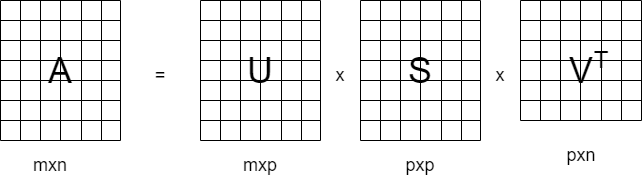
\includegraphics[width=0.8\textwidth]{Bilder_Stand_der_Technik/matrix_svd.png}}
    \caption{\label{figure:Matrix_SVD}SWZ-Matrize}
\end{figure}
\noindent
Wobei m die Anzahl der Begriffe im Wörterbuch, n die Anzahl der Dokumente im Korpus und p die Summe der Themen im Korpus ist, die der Anzahl der Wörter entspricht.\\\\
Nach dem Theorem von Eckart-Young reduziert die \ac{SWZ} das Rauschen und die Spärlichkeit der ursprünglichen Matrix, indem sie durch eine Matrix derselben Dimensionalität, aber niedrigeren Rangs ersetzt wird, in der nur die wichtigsten Informationen erhalten bleiben. \cite{eckart_approximation_1936}\\\\
Die U-Matrix enthält die Term-Themen-Matrix. 
Sie wird auch als linke singuläre Vektormatrix bezeichnet, da sie die Zeilenvektoren enthält, die von links mit der Spaltenvektormatrix zu multiplizieren sind. 
Die U-Matrix spiegelt die gegenseitige Korrelation von Wörtern und Themen auf der Grundlage des gemeinsamen Auftretens von Wörtern im selben Dokument wider. 
Vor der Trunkierung (Entfernung der Spalten) ist sie quadratisch. 
Die Anzahl der Spalten und Zeilen in ihr entspricht der Anzahl der Wörter im Wörterbuch (m). 
Vor der Trunkierung ist die Anzahl der Themen (p) gleich der Anzahl der Wörter. 
Die U-Matrix enthält als Spalten Vektoren der Themen für alle Wörter des Korpus. 
Das bedeutet, dass sie verwendet werden kann, um einen Wort-Dokument-Vektor (\ac{TF-IDF}-Vektor oder \ac{BOW}-Vektor) in einen Themen-Dokument-Vektor umzuwandeln. 
Um einen neuen \glqq topic-document\grqq{}-Vektor zu erhalten, multipliziert man einfach die U-Matrix \glqq topic-word\grqq{} mit einem beliebigen \glqq word-document\grqq{}-Vektor. 
Der Punkt ist, dass die Gewichte (Scores) in den Zellen der U-Matrix die Bedeutung der Wörter für die Themen widerspiegeln. \cite{manning_introduction_2008}\\\\
Die quadratische diagonale S-Matrix (Sigma-Matrix) enthält die Singulärwerte (Eigenwerte) des Themas. 
Diese singulären Werte geben an, wie viel Information in jeder Dimension des neuen semantischen (Themen-)Vektorraums enthalten ist. 
In der diagonalen Matrix befinden sich Werte, die nicht Null sind, nur auf der Diagonalen von der linken oberen Ecke bis zur rechten unteren Ecke. 
Alle anderen Positionen in der S-Matrix enthalten Nullen. 
Und die Dimensionen (Themen) sind so angeordnet, dass die erste Dimension die meisten Informationen (erklärbare Varianz) über den Fall enthält \cite{deerwester_indexing_1990}.
Wenn es also notwendig ist, das Themenmodell abzuschneiden, kann man mit den Messungen von unten rechts beginnen und sich nach links bewegen. 
Und dann aufhören, diese singulären Werte auf Null zu setzen, wenn der Fehler des thematischen Modells eine signifikante Auswirkung auf den Gesamtfehler der \ac{NLP}-Pipeline haben wird.\\\\
Die $V^{T}$-Matrix \glqq Dokument-Dokument\grqq{} enthält als Spalten die rechten singulären Vektoren und gibt Aufschluss über die gemeinsamen Bedeutungen von Dokumenten, da sie die Häufigkeit der Verwendung der gleichen Themen in Dokumenten in dem neuen semantischen Modell von Dokumenten misst. 
Es enthält so viele Zeilen (p) und Spalten, wie es Dokumente im Korpus gibt. \cite{lane_natural_2019}\\\\
Nachdem die singuläre Zerlegung abgeschlossen ist, müssen die Themen so gekürzt werden, dass sie die Bedeutung der Dokumente wiedergeben. 
Dabei müssen die Elemente der Matrix S in absteigender Reihenfolge sortiert werden. 
In diesem Fall kann die Formel in einer anderen Form geschrieben werden:
\begin{equation}
    A_{k} = U_{k} S_{k} V_{k}^T
    \eqlabel{eq-trunkierte-swz}{Trunkierte SWZ-Matrix}
\end{equation}
Dabei sind $U_{k}$ und $V_{k}$ Matrizen, die durch Extraktion der ersten k Spalten aus den Matrizen U bzw. V gewonnen werden.
\begin{figure}[H]
    \centering
    \fbox{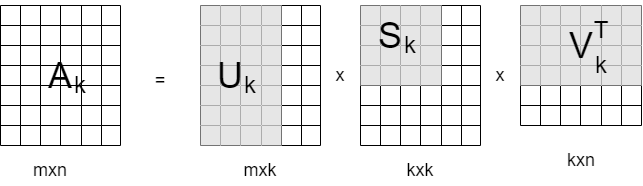
\includegraphics[width=0.8\textwidth]{Bilder_Stand_der_Technik/trun_svd.png}}
    \caption{\label{figure:Trun_SVD}Trunkierte SWZ-Matrize}
\end{figure}
\noindent
Im latent-semantischen Modell kann also jeder Text und jeder Begriff durch Vektoren in einem reduzierten Raum der Dimension k - dem Themenraum - dargestellt werden. 
Diese \ac{SWZ} wird als parsimonious bezeichnet, weil sie in dem Fall, in dem k viel kleiner als m, n und p ist, eine erhebliche Kompression der ursprünglichen Information ermöglicht. 
Komprimierung ist in dem Sinne zu verstehen, dass ein Teil der von der ursprünglichen Matrix übermittelten Informationen verloren geht und nur die wichtigsten (dominanten) Informationen erhalten bleiben. 
Der Informationsverlust entsteht durch die Vernachlässigung kleiner Singulärzahlen \cite{deerwester_indexing_1990}.
Je mehr Singulärzahlen verworfen werden, d. h. je kleiner k, desto größer ist dieser Verlust. 
Mit anderen Worten: Der Informationsverlust ist umso größer, je niedriger der Rang der approximierenden Matrix ist. 
In diesem Fall gehen zunächst die nicht signifikanten Werte verloren, wodurch die dominanten Werte der Matrix erhöht werden. \cite{lane_natural_2019}\\\\
Der \ac{SWZ}-Algorithmus, das Herzstück von \ac{LSA}, erkennt, ob Wörter immer nebeneinander vorkommen und fasst sie im Betreff zusammen. 
Auf diese Weise kann er die Anzahl der Messungen ohne zusätzlichen Aufwand reduzieren. 
\ac{LSA} (\ac{SWZ}) ist eine großartige Methode, um Wort-Dokument-Matrizen zu komprimieren und potenzielle zusammengesetzte Wörter oder N-Gramme für die Pipeline zu erkennen. 
\ac{LSA} reduziert die Anzahl der Messungen und hilft so, Übertraining zu vermeiden. 
Sie führt eine Verallgemeinerung auf der Grundlage eines kleinen Datensatzes durch, indem sie eine lineare Beziehung zwischen den Worthäufigkeiten annimmt. \cite{jurafsky_speech_2009}\\\\
\ac{LSA}s können auch für die semantische Suche verwendet werden. 
Eine semantische Suche (semantic search) ist eine Art der Volltextsuche, die die Bedeutung der Wörter in der Anfrage und der gesuchten Dokumente berücksichtigt. 
Durch die Verwendung von Themenvektoren ist es möglich, die Bedeutung von Wörtern, Dokumenten, Aussagen und Korpora zu vergleichen. 
Es ist möglich, Cluster von ähnlichen Dokumenten und Aussagen zu finden. 
Mit Themenvektoren wird der Abstand zwischen Dokumenten nicht nur auf der Grundlage der in ihnen verwendeten Wörter betrachtet, sondern auf der Grundlage von Wörtern, die der Bedeutung entsprechen. 
Semantische Suchen mit Themenvektoren beschränken sich nicht nur auf die Suche nach Schlüsselwörtern und Relevanzrankings, die allein auf der Auswahl von Wörtern oder Vokabeln basieren. 
Sie können verwendet werden, um Dokumente zu finden, die für die Anfrage relevant sind, und nicht nur solche, die gut zu den Wortstatistiken passen. 
Dazu muss die Suchanfrage des Nutzers zunächst mit denselben Attributen vektorisiert werden wie die Dokumentenvektorisierung. 
Dann kann \ac{SWZ} verwendet werden, um die Dimensionalität des Abfragevektors auf die gleichen Dimensionen wie die der Dokumentvektoren zu reduzieren. 
Anschließend kann der Kosinuskoeffizient zwischen dem Abfragevektor und den Dokumentvektoren berechnet werden, um festzustellen, welche Dokumente der Abfrage am nächsten liegen. 
\ac{LSA} und \ac{SWZ} können also zum Aufspüren versteckter Themen in Textdokumenten sowie zur semantischen Suche in großen Dokumentensammlungen verwendet werden. \cite{lane_natural_2019}\\\\
Es gibt viele Python-Bibliotheken und -Werkzeuge für die Implementierung von \ac{LSA} und \ac{SWZ}. 
Eine der beliebtesten Bibliotheken für Matrix- und Singulärzerlegung ist NumPy. 
NumPy erleichtert die Durchführung von Matrixoperationen und verfügt über eine Funktion zur Singulärzerlegung: \textit{numpy.linalg.svd()} \cite{numpy}.
Zusammen mit anderen Bibliotheken wie \textit{Pandas} und \textit{Scikit-learn} kann \ac{LSA} effizient durchgeführt werden. 
Um \ac{LSA} zu starten, müssen die Textdaten mit Hilfe des \ac{TF-IDF}-Modells vektorisiert werden, wie zuvor beschrieben. 
Dann muss eine singuläre Zerlegung der Term-Dokument-Matrix mit \textit{numpy.linalg.svd()} durchgeführt werden. 
Danach kann eine bestimmte Anzahl von Hauptkomponenten (Topics) ausgewählt werden, die zur Darstellung der Dokumente verwendet werden. 
Dies kann durch die Auswahl der Komponenten mit den höchsten Singulärwerten geschehen. 
Anhand dieser Komponenten kann dann die Nähe zwischen den Dokumenten bestimmt werden.\\\\ 
\textit{Scikit-learn} bietet auch eine \textit{TruncatedSVD}-Klasse, mit der eine Truncated-\ac{SVD} durchgeführt werden kann, um nur die ausgewählten Hauptkomponenten zu erhalten. 
Diese Klasse erleichtert die Durchführung von \ac{LSA} auf großen Dokumentenkorpora und verfügt über zusätzliche Funktionen wie Datenverarbeitung und Normalisierung sowie automatische Auswahl der Anzahl der Komponenten auf der Grundlage des Prozentsatzes der erklärten Varianz. \cite{scikit-learn}
\subsection{Ansätze für die Erstellung eines Chatbots}\label{sec:ansaetze_erstellung_chatbots}
Derzeit gibt es vier Hauptansätze für die Erstellung eines Chatbots \cite{lane_natural_2019}:
\begin{itemize}
    \item Musterabgleich: Musterabgleich und Antwortvorlagen (vorgefertigte Antworten)
    \item Grounding: logische Wissensgraphen und das Ziehen von Schlussfolgerungen aus diesen basierend auf diesen Graphen
    \item Suche: Abrufen von Text
    \item Generierungsmethoden: Statistik und maschinelles Lernen
\end{itemize}
Die vier grundlegenden Ansätze zur Erstellung von Chatbots lassen sich kombinieren, was zu benutzerfreundlicheren Chatbots führt. 
Eine Vielzahl von Anwendungen nutzen alle vier grundlegenden Methoden. 
Hybride Chatbots unterscheiden sich hauptsächlich darin, wie genau sie diese Ansätze kombinieren und wie viel Gewicht auf jeden einzelnen Ansatz gelegt wird.
\subsubsection{Musterabgleich}
Bei den ersten Chatbots basierte die Antwort auf die Nachricht eines Benutzers auf einem Mustervergleich. 
Diese Chatbots suchen nach Mustern im eingehenden Text und geben eine feste (gemusterte) Antwort, wenn eine Übereinstimmung gefunden wird \cite{woudenberg_chatbot_2014}.\\\\
Solche rudimentären Dialogsysteme sind vor allem in automatisierten Benutzerunterstützungssystemen mit interaktiven Sprachmenüs nützlich, wo es möglich ist, das Gespräch an einen Menschen weiterzuleiten, wenn der Chatbot keine Antwortmuster mehr hat.\\\\
Da es viele \ac{NLP}-Dienstprogramme in Python-Paketen gibt, ist es möglich, komplexere Chatbots auf der Grundlage von Mustervergleichen zu erstellen, indem man die Bot-Logik nach und nach direkt in Python mit regulären Ausdrücken und Suchmustern aufbaut.\\\\
1995 machte sich Richard Wallace daran, einen allgemeinen Rahmen für die Erstellung von Chatbots auf der Grundlage des Pattern-Matching-Ansatzes zu schaffen. Zwischen 1995 und 2002 schuf seine Entwicklergemeinschaft die \ac{AIML} zur Beschreibung von Mustern und Chatbot-Antworten.\\\\
\ac{AIML} ist eine deklarative Sprache, die auf dem \ac{XML}-Standard basiert, der die Sprachkonstrukte und Datenstrukturen einschränkt, die im Bot verwendet werden dürfen. \cite{noauthor_aiml_nodate}
Ein Chatbot, der auf \ac{AIML} basiert, sieht folgendermaßen aus:
\begin{figure}[H]
    \centering
    \fbox{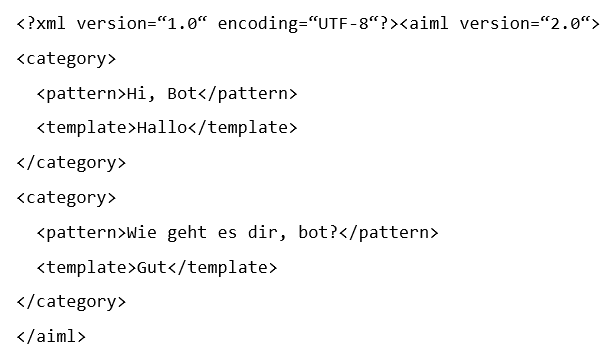
\includegraphics[width=0.8\textwidth]{Bilder_Stand_der_Technik/aiml_bot.png}}
    \caption{\label{figure:Aiml_Bot}AIML-Chatbot}
\end{figure}
\noindent
Eine der Einschränkungen von \ac{AIML} ist die Art der Muster, die abgeglichen werden können und auf die reagiert wird. 
Der \ac{AIML}-Kern (Pattern Matching Engine) reagiert nur auf Eingabetext, der einem vom Entwickler manuell vorgegebenen Muster entspricht. 
Unscharfe Suchanfragen, Smileys, Satzzeichen, Tippfehler oder falsch geschriebene Wörter sind nicht erlaubt, es findet kein automatischer Abgleich statt. 
In \ac{AIML} müssen alle Synonyme manuell einzeln beschrieben werden.
\subsubsection{Grounding}
Die Grounding-Methode ist ein Ansatz zur Erstellung eines Chatbots auf der Grundlage logischer Wissensgraphen und der Durchführung von Schlussfolgerungen auf der Grundlage dieser Graphen. \cite{diana_conversational_2011}
Sie wird verwendet, um natürliche Sprache zu verarbeiten und sie dem Verständnis des Bots zuzuordnen. Das Wesentliche an der Grounding-Methode ist, dass der Chatbot nicht nur die Textnachrichten, sondern auch den Kontext und die Umgebung verarbeitet, um Anfragen besser zu verstehen und zu beantworten. 
Durch die Extraktion von Informationen wird ein Netz von Verbindungen oder Fakten geschaffen. Dieses Netz logischer Verbindungen zwischen Entitäten - ein Graph oder eine Wissensbasis - kann die Grundlage für die Antworten des Chatbots bilden.\\\\
Ein Beispiel für eine Grounding-Methode ist die Verwendung eines Wissensgraphen zur Beschreibung der Umgebung. 
Ein Wissensgraph enthält Informationen über die Objekte, mit denen der Bot interagieren kann und die Beziehungen zwischen ihnen. 
Ein Wissensgraph könnte zum Beispiel Informationen über ein Glas auf einem Tisch und das darin befindliche Wasser enthalten. 
Wenn ein Benutzer eine Frage stellt, verwendet der Chatbot den Wissensgraphen, um den Kontext der Anfrage zu verstehen und die am besten geeignete Antwort abzuleiten. 
Wenn ein Benutzer zum Beispiel fragt: \glqq{}Wie hoch ist die Temperatur des Wassers in dem Glas auf dem Tisch?\grqq{}, kann der Chatbot Informationen aus dem Wissensgraphen verwenden, um die Frage zu beantworten.\\\\
Ein solcher Wissensgraph kann abgeleitet werden, um Fragen über die in dieser Wissensbasis enthaltene Welt zu beantworten und anschließend können auf der Grundlage der logischen Antworten die Werte der in den Antworten enthaltenen Template-Variablen ausgefüllt werden, um natürlichsprachliche Antworten zu erstellen. 
Ursprünglich wurden auf diese Weise Systeme zur Beantwortung von Fragen eingerichtet, wie z. B. der Watson-Bot von IBM (heutzutage wird für ähnliche Systeme jedoch die Informationssuchemethode verwendet). 
Der Wissensgraph stellt eine Art \glqq{}Erdung\grqq{} des Chatbots in der realen Welt dar.\\\\
Die Erstellung von Chatbots auf der Grundlage von \glqq{}Grounding\grqq{} eignet sich hervorragend für Chatbots, die Fragen generieren, bei denen das zur Beantwortung einer Frage erforderliche Wissen in einer umfangreichen Wissensbasis enthalten ist, die aus einer offenen Datenbank (z. B. Wikidata, Open Mind Common Sense oder DBpedia) bezogen werden kann.\\\\
Einer der Hauptvorteile der Grounding-Methode besteht darin, dass sie sich an ein sich veränderndes Umfeld anpassen kann. 
Wenn der Benutzer zum Beispiel ein Glas Wasser von einem Tisch auf einen anderen stellt, wird der Wissensgraph automatisch aktualisiert, um diese Änderung widerzuspiegeln.\\\\
Die Grounding-Methode hat jedoch auch ihre Grenzen. 
So kann es vorkommen, dass bei der Verarbeitung großer Informationsmengen Zusammenhänge nicht berücksichtigt werden und dem Bot möglicherweise verborgen bleiben.\\\\
Insgesamt ist die Grounding-Methode ein effektiver Ansatz zur Erstellung wissensbasierter Chatbots. 
Sie ermöglicht es dem Bot, Benutzeranfragen besser zu verstehen und eine genauere Antwort zu geben.
\subsubsection{Suche}
Die Informationssuchemethode ist eine der Methoden zum Aufbau von Chatbots, die auf der Extraktion von Informationen aus einer großen Menge von Textinformationen basiert. 
Die Hauptidee der Informationssuchemethode ist die Analyse des Eingabetextes (Benutzeranfrage), die Auswahl von Schlüsselwörtern und Phrasen daraus und die anschließende Suche nach den relevantesten Informationen in der Wissensdatenbank oder in offenen Quellen. \cite{diana_conversational_2011}\\\\
Die Wissensbasis kann auch eine Art \glqq{}Gesprächsprotokoll\grqq{} sein, in Form von Aussage-Antwort-Paaren. 
Dabei sucht der Bot nach früheren Aussagen in den Protokollen früherer Unterhaltungen. 
Der Bot kann nicht nur in den Protokollen seiner eigenen Gespräche suchen, sondern auch in beliebigen Transkripten von Gesprächen zwischen Menschen, Gesprächen zwischen Menschen und Bots oder sogar Gesprächen zwischen Bots.
Aber wie immer gilt: je besser die Eingabedaten, desto besser das Ergebnis. 
Daher ist es notwendig, die Datenbank früherer Gespräche sorgfältig zu säubern und zu organisieren, damit der Bot nach einem qualitativ hochwertigen Gespräch sucht und es dann imitiert.\\\\
Für die Umsetzung der Informationssuchemethode werden verschiedene Algorithmen und Techniken verwendet, z. B. Indizierung und Schlagwortsuche, Kontextsuche, Textanalyse mit Hilfe von maschinellen Lernverfahren usw. 
Die Informationssuchemethode kann in Python mit verschiedenen Bibliotheken und Tools wie \ac{NLTK}, Scikit-learn und Gensim implementiert werden.\\\\
Einer der ersten Schritte bei der Implementierung einer Informationssuchemethode in Python ist die Vorbereitung der Daten. 
Dies erfordert Tokenisierung, Lemmatisierung und die Entfernung von Stopp-Wörtern. 
Als nächstes muss ein Index auf der Grundlage von Schlüsselwörtern erstellt werden. 
Der Index kann auf der Grundlage von Bag-of-Words oder \ac{TF} und \ac{IDF} (TF-IDF-Modelle) erstellt werden. 
Sobald der Index erstellt ist, kann eine Stichwortsuche durchgeführt werden. 
Dazu muss die Benutzeranfrage in einen Vektor umgewandelt und mit den Dokumentvektoren im Index verglichen werden. 
Dies kann mit Hilfe der Scikit-learn-Bibliothek erfolgen \cite{scikit-learn}.
Sobald die relevantesten Dokumente gefunden wurden, können sie in eine Rangfolge gebracht und als Antwort auf die Benutzeranfrage angezeigt werden.\\\\
Der Vorteil der Informationssuchemethode besteht darin, dass sie ein schnelles und genaues Auffinden der gewünschten Informationen ermöglicht, insbesondere wenn die Wissensbasis gut strukturiert ist und genügend Informationen enthält. 
Ein Nachteil dieser Methode ist jedoch, dass sie den Kontext der Anfrage nicht berücksichtigt und nicht immer eine vollständige und genaue Antwort auf die Frage des Nutzers liefert. 
Wenn die Aussage semantisch mit der vom Bot zu beantwortenden übereinstimmt, ist es möglich, die Antwort wortwörtlich und ohne Änderungen wiederzuverwenden. 
Aber selbst wenn die Datenbank alle möglichen Benutzeräußerungen enthält, wird der Bot die Persönlichkeiten der Personen widerspiegeln, die diese Äußerungen machen. 
Wenn die Antworten konsistent sind und von einer Vielzahl von Personen stammen, ist das gut. 
Problematisch wird es jedoch, wenn die Äußerung, auf die der Bot reagieren soll, vom Gesamtkontext des jeweiligen Gesprächs oder von den Umständen in der Umgebung abhängt, die sich seit der Erstellung des Dialogkorpus geändert haben können.\\\\
Beispielsweise sollte der Bot auf die Frage \glqq{}Wie spät ist es?\grqq{} nicht die von der Person gegebene Antwort, sondern die am besten geeignete Aussage aus der Datenbank verwenden. 
Diese Antwort funktioniert nur, wenn die Zeit, zu der die Frage gestellt wurde, mit der Zeit übereinstimmt, zu der die passende Äußerung aus der Datenbank aufgezeichnet wurde. 
Neben dem natürlichsprachlichen Text der Äußerung müssen auch ähnliche Informationen über die Zeit - der Kontext (Zustand) - erfasst und verglichen werden. 
Sie spielt vor allem dann eine wichtige Rolle, wenn die Semantik der Äußerung auf eine aktive Veränderung des im Kontext (Wissensbasis des Chatbots) erfassten Zustands hinweist.\\\\
Um den Zustand (Kontext) in einem Chatbot auf der Grundlage der Informationssuche zu berücksichtigen, kann etwas Ähnliches für einen Chatbot mit Musterabgleich durchgeführt werden, da die Auflistung einer Liste von Benutzeraussagen nur eine andere Art ist, ein Muster zu beschreiben. 
Dies auch ist der Ansatz von Amazon Lex \cite{amazon_lex} und Google Dialogflow \cite{dialogflow_chawla}. 
Anstatt ein starres Muster zu beschreiben, um den Befehl des Benutzers zu erfassen, können der Dialogflow-Engine einfach ein paar Beispiele geliefert werden. 
So wie jedes Muster im Chatbot auf der Grundlage der Musterzuordnung einem Zustand zugeordnet wurde, muss auch hier nur die Aussage-Antwort-Beispielpaare mit dem genannten Zustand verknüpft werden.\\\\
Der suchbasierte Chatbot indiziert also den Korpus der Dialoge, so dass er leicht frühere Aussagen finden kann, die derjenigen ähnlich sind, auf die er antworten muss und antwortet dann mit einer der passenden Aussagen aus dem Korpus, die er sich \glqq{}gemerkt\grqq{} und für eine schnelle Suche indiziert hat. 
Im Allgemeinen ist die Methode der Informationssuche eine der gängigsten und beliebtesten Methoden zum Aufbau von Chatbots, die in verschiedenen Bereichen wie Wirtschaft, Medizin, Tourismus und vielen anderen eingesetzt werden.
\subsubsection{Generierungsmethoden}
Generierungsmethoden sind einer der wichtigsten Ansätze bei der Entwicklung von Chatbots auf der Grundlage künstlicher Intelligenz. 
Sie ermöglichen es Chatbots, Textantworten auf der Grundlage der Analyse der eingehenden Nachricht und des Kontextes des Dialogs zu generieren. 
Die folgenden Generierungsmodelle sind nützlich, um einen kreativen Chatbot zu erstellen, der Dinge sagen kann, die noch niemand zuvor gesagt hat:
\begin{itemize}
    \item Sequenz-zu-Sequenz-Konvertierungsmodelle: Modelle, die darauf trainiert sind, Antworten auf der Grundlage von Eingabesequenzen zu generieren;
    \item \ac{RBM}: Markov-Ketten, die so trainiert werden, dass sie die \glqq{}Energie\grqq{}-Funktion minimieren \cite{chatbot_development_sharma};
    \item \ac{GAN}: statistische Modelle, die darauf trainiert sind, einen Experten, der die Qualität eines Gesprächs bewertet, zu täuschen. \cite{li_adversarial_2017}
\end{itemize}
Die Vorteile des Einsatzes der Generierungsmethoden:
\begin{itemize}
    \item Flexibilität: Generative Methoden können für eine breite Palette von Aufgaben eingesetzt werden, einschließlich Texterstellung, Sprachübersetzung, Verarbeitung natürlicher Sprache und mehr.
    \item Automatisierung: Generative Methoden können auf großen Datensätzen trainiert werden, wodurch die Erstellung von Inhalten automatisiert werden kann.
    \item Qualität: Generative Methoden zeigen eine hohe Qualität bei der Textgenerierung, Sprachübersetzung und anderen Aufgaben der natürlichen Sprachverarbeitung, wenn sie auf einem ausreichend großen Datensatz trainiert werden.
    \item Schnelligkeit: Generative Methoden können schneller arbeiten als Menschen, was die Erstellung von Inhalten mit großer Geschwindigkeit ermöglicht.
\end{itemize}
Die Nachteile der generativen Methoden:
\begin{itemize}
    \item Große Datenmengen für das Training: Generative Methoden benötigen große Datenmengen für das Training, was bei einigen Aufgaben schwierig sein kann, insbesondere wenn nur ein kleiner Datensatz zur Verfügung steht.
    \item Sicherheitsrisiken: Generative Methoden können Inhalte erzeugen, die möglicherweise falsch, unvollständig oder irreführend sind. Dies kann zu Sicherheitsrisiken führen, wenn der generierte Inhalt für wichtige Entscheidungen verwendet wird.
    \item Unterstützungsbedarf: Generative Methoden können erhebliche Unterstützung benötigen, um effektiv zu sein. Dies kann die Modellabstimmung, die Auswahl optimaler Parameter und die Optimierung der Modellleistung auf einer bestimmten Hardwarekonfiguration umfassen.
    \item Modellbeschränkungen: Generative Methoden können Beschränkungen hinsichtlich der Arten von Inhalten haben, die sie erzeugen können, insbesondere wenn sie nur auf bestimmte Datentypen trainiert wurden.
\end{itemize}
Eine der beliebtesten Methoden zur Texterstellung ist die sequence-to-sequence-Methode (seq2seq). 
Die seq2seq-Methode basiert auf \ac{RNN}, die die Simulation von Datenfolgen ermöglichen. 
Sie besteht aus zwei Hauptteilen: einem Encoder und einem Decoder. 
Ein Encoder empfängt eine Wortfolge und baut daraus einen Kontextvektor auf, der Informationen über die Eingabedaten enthält. 
Der Decoder erhält diesen Vektor als Eingabe und beginnt mit der Generierung einer Folge von Antwortnachrichten, wobei er schrittweise den Kontext und die zuvor generierten Wörter berücksichtigt. \cite{seq2seq_alammar}\\\\
Einer der Hauptvorteile der seq2seq-Methode ist ihre Fähigkeit, qualitative und grammatikalisch korrekte Textantworten zu generieren, einschließlich Antworten, die nicht in den Trainingsdaten enthalten waren. 
Sie kann auch mit langen Sequenzen umgehen, was sie ideal für die Generierung von Antworten in Dialogsystemen macht. 
Darüber hinaus kann die seq2seq-Methode in einer Vielzahl von Anwendungen eingesetzt werden, z. B. in der maschinellen Übersetzung, der Spracherkennung und anderen.\\\\
Die seq2seq-Methode hat jedoch ihre Nachteile. 
Sie erfordert große Datenmengen zum Trainieren und Verarbeiten sowie erhebliche Rechenressourcen. 
Dies kann die Anwendung der Methode bei einigen Anwendungen einschränken. 
Wenn der Trainingsdatensatz nicht eine ausreichend große Bandbreite möglicher Antworten repräsentiert, kann das Modell außerdem dazu neigen, vorhersehbare oder falsche Antworten zu erzeugen.\\\\
Die Implementierung der seq2seq-Methode in Python kann mit der TensorFlow-Bibliothek erfolgen, die eine Reihe von Werkzeugen für den Aufbau und das Training neuronaler Netze bietet. 
In TensorFlow kann man die vortrainierten seq2seq-Modelle verwenden oder ein eigenes Modell erstellen, indem die Architektur und die Trainingsparameter des Netzwerks konfiguriert wird. \cite{tensorflow}
\subsection{Mehrschichtiges Perzeptron für ein Mehrklassen-Klassifizierungsproblem}
Ein \ac{MLP} ist eine neuronale Netzwerkarchitektur, die aus mehreren Schichten von Neuronen besteht und für Klassifizierungs- und Regressionsaufgaben verwendet werden kann. 
Mehrschichtige Perzeptronen sind Arten von neuronalen Netzen, die bidirektional sind, da sie die Eingabedaten vorverteilen und die Gewichte zurückverteilen. 
Ein mehrschichtiges Perzeptron hat eine Eingabeschicht und eine Ausgabeschicht mit einer oder mehreren versteckten Schichten. 
Bei \ac{MLP} sind alle Neuronen einer Schicht mit allen Neuronen der nächsten Schicht verbunden. 
Die Eingabeschicht empfängt Eingangssignale und die gewünschte Aufgabe wird von der Ausgabeschicht ausgeführt. 
Die versteckten Schichten sind für alle Berechnungen zuständig. 
Die Architektur des mehrschichtigen Perzeptrons sieht folgendermaßen aus:
\begin{figure}[H]
    \centering
    \fbox{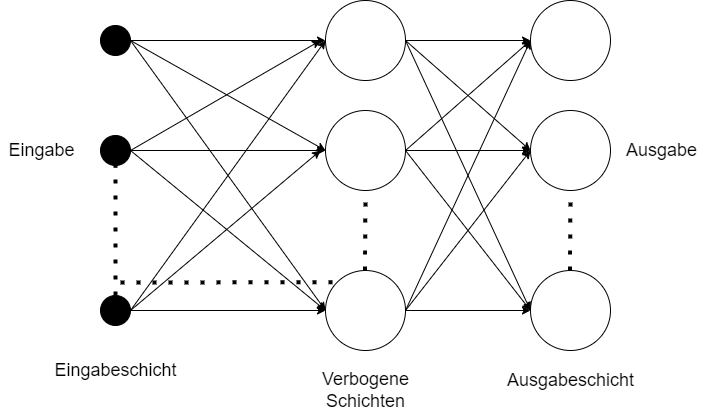
\includegraphics[width=0.8\textwidth]{Bilder_Stand_der_Technik/mehrschicht_perc.png}}
    \caption{\label{figure:Mehrschichtiges_Perzeptron}Mehrschichtiges Perzeptron}
\end{figure}
\noindent
Für ein Mehrklassen-Klassifizierungsproblem kann ein \ac{MLP} mit einer Verlustfunktion wie der kategorialen Kreuzentropie (Categorical Crossentropy) trainiert werden. 
Zunächst muss ein \ac{MLP} über eine Eingabeschicht verfügen, die die Merkmale eines Objekts aufnimmt, und eine Ausgabeschicht, die die Wahrscheinlichkeiten für die Zugehörigkeit des Objekts zu den einzelnen Klassen ausgibt. 
Die Dimensionalität der Ausgabeschicht muss der Anzahl der zu klassifizierenden Klassen entsprechen \cite{goodfellow_deep_2016}.
Außerdem können zwischen der Eingabe- und der Ausgabeschicht mehrere verborgene Schichten liegen, die nichtlineare Transformationen der Eingabedaten durchführen, so dass das \ac{MLP}-Modell komplexe Beziehungen zwischen Objektmerkmalen und Klassen erfassen kann. 
Jedes Neuron im \ac{MLP} nimmt als Eingabe die gewichtete Summe der Neuronenausgaben der vorherigen Schicht, fügt eine Vorspannung hinzu und durchläuft dann eine Aktivierungsfunktion. 
Die Aktivierungsfunktion wird verwendet, um dem \ac{MLP} Nichtlinearität hinzuzufügen und kann z. B. sigmoid-Funktion oder ReLU sein.
Beim \ac{MLP}-Training mit Gradientenabstieg werden die Gewichte und Vorspannungen der Neuronen bei jeder Trainingsiteration aktualisiert, wobei der Wert der Verlustfunktion minimiert wird. \cite{geron_hands-machine_2019}\\\\
Die kategoriale Kreuzentropie ist eine Verlustfunktion, die für die Klassifizierung mehrerer Klassen verwendet wird und die Diskrepanz zwischen den wahren Klassenbezeichnungen und den vorhergesagten Klassenwahrscheinlichkeiten misst. 
Daher kann \ac{MLP} nach dem Training zur Klassifizierung neuer Objekte verwendet werden, indem die Objektmerkmale durch \ac{MLP} geleitet werden und die Ausgabewahrscheinlichkeiten für jede Klasse ermittelt werden und dann die Klasse mit der höchsten Wahrscheinlichkeit als vorhergesagte Klassenbezeichnung ausgewählt wird. \cite{aggarwal_neural_2018}\\\\
Die Theorie hinter der kategorialen Kreuzentropie ist die Informationstheorie und die Messung der Unsicherheit. 
Angenommen, es gibt ein System, das mit einem probabilistischen Modell beschreiben werden muss. 
Dieses System habe N mögliche Ergebnisse, die jeweils mit den Wahrscheinlichkeiten $p_{1}$, $p_{2}$, ..., $p_{N}$ auftreten können, wobei $\sum_i p_i = 1$ und $p_i\geq0$ für i = 1, 2, ..., N. 
Dann kann die Entropie H des Systems wie folgt definiert werden: 
\begin{equation}
    H = -\sum (p_{i}*\log_{2}{p_{i}})
    \eqlabel{eq-entropie}{Entropie H}
\end{equation}
Dabei wird $\sum$($p_{i}$* $\log_{2}{p_{i}}$) über i von 1 bis N genommen \cite{koech_cross-entropy_2022}. 
Diese Formel zeigt, dass die Entropie des Systems ein Maß für die Ungewissheit oder Unsicherheit bei der Wahl eines der möglichen Ergebnisse ist.\\\\
Wenn die kategoriale Kreuzentropie als Verlustfunktion für ein Mehrklassen-Klassifizierungsproblem verwendet wird, wird erwartet, dass das trainierte Modell einen Ausgabewahrscheinlichkeitsvektor hat, bei dem jedes Element des Vektors einer der Klassen entspricht. 
Je unsicherer der Modellausgabevektor für ein bestimmtes Beispiel ist, desto höher ist der Wert der kategorialen Kreuzentropie. 
Umgekehrt ist der Wert der kategorialen Kreuzentropie gleich Null, wenn das Modell eine Klasse für ein bestimmtes Beispiel genau vorhersagt.
Beim Training von Klassifizierungsmodellen für Aufgaben des maschinellen Lernens mit mehreren Klassen wird daher versucht, den Wert der kategorialen Kreuzentropie zwischen dem Ausgabevektor des Modells und der richtigen Klasse für jedes Eingabebeispiel zu minimieren. 
Zu diesem Zweck wird ein Optimierungsverfahren verwendet, z. B. den Gradientenabstieg, um die Gewichte und Verzerrungen des Modells bei jeder Trainingsiteration zu aktualisieren. \cite{raschka_python_2017}\\\\
In Keras kann die kategoriale Kreuzentropie als Verlustfunktion für verschiedene Modelltypen wie mehrschichtige Perzeptronen, faltungsneuronale Netze und rekurrente neuronale Netze verwendet werden. 
Es handelt sich um eine Standardverlustfunktion für Mehrklassen-Klassifizierungsprobleme \cite{geron_hands-machine_2019}.
Bei der Verwendung der kategorialen Kreuzentropie in Keras können auch verschiedene Parameter wie Klassengewichte und Modellbewertungsmetriken angepasst werden, um genauere Klassifizierungsergebnisse zu erhalten. 
Somit ist die kategoriale Kreuzentropie ein wichtiges Werkzeug beim maschinellen Lernen zur Lösung von Klassifizierungsproblemen mit mehreren Klassen. 
Ihre Verwendung ermöglicht es, Modelle zu trainieren, die Eingabebeispiele genau klassifizieren und eine hohe Genauigkeit bei Klassifizierungsaufgaben erreichen können.

\endinput